\documentclass{article}
% if you need to pass options to natbib, use, e.g.:
     \PassOptionsToPackage{numbers, compress}{natbib}
% before loading neurips_2020

% ready for submission
% \usepackage{neurips_2020}

% to compile a preprint version, e.g., for submission to arXiv, add add the
% [preprint] option:
%     \usepackage[preprint]{neurips_2020}

% to compile a camera-ready version, add the [final] option, e.g.:
%     \usepackage[final]{neurips_2020}

% to avoid loading the natbib package, add option nonatbib:
     \usepackage[nonatbib]{neurips_2020}

\usepackage[utf8]{inputenc} % allow utf-8 input
\usepackage[T1]{fontenc}    % use 8-bit T1 fonts
\usepackage{hyperref}       % hyperlinks
\usepackage{url}            % simple URL typesetting
\usepackage{booktabs}       % professional-quality tables
\usepackage{amsfonts}       % blackboard math symbols
\usepackage{nicefrac}       % compact symbols for 1/2, etc.
\usepackage{microtype}      % microtypography
\usepackage{amsmath}
%Graphs
\usepackage{tikz}
\usepackage{pgfplots}
\usepackage[export]{adjustbox}
\usepackage{xcolor,colortbl}
\usepackage[capposition=top]{floatrow}
\hypersetup{
	colorlinks,
	linkcolor = {red!50!black},
	citecolor = {blue!50!black},
	urlcolor = {blue!80!black}
}

\usepackage{lscape}
\usepackage{longtable}

\title{Evaluation of Machine Learning in Empirical Asset Pricing}

% The \author macro works with any number of authors. There are two commands
% used to separate the names and addresses of multiple authors: \And and \AND.
%
% Using \And between authors leaves it to LaTeX to determine where to break the
% lines. Using \AND forces a line break at that point. So, if LaTeX puts 3 of 4
% authors names on the first line, and the last on the second line, try using
% \AND instead of \And before the third author name.

\author{%
  David S.~Hippocampus\thanks{Use footnote for providing further information
    about author (webpage, alternative address)---\emph{not} for acknowledging
    funding agencies.} \\
  Department of Computer Science\\
  Cranberry-Lemon University\\
  Pittsburgh, PA 15213 \\
  \texttt{hippo@cs.cranberry-lemon.edu} \\
  % examples of more authors
  % \And
  % Coauthor \\
  % Affiliation \\
  % Address \\
  % \texttt{email} \\
  % \AND
  % Coauthor \\
  % Affiliation \\
  % Address \\
  % \texttt{email} \\
  % \And
  % Coauthor \\
  % Affiliation \\
  % Address \\
  % \texttt{email} \\
  % \And
  % Coauthor \\
  % Affiliation \\
  % Address \\
  % \texttt{email} \\
}

\begin{document}

\maketitle

\begin{abstract}
  Several recent studies have claimed that machine learning methods provide superior predictive accuracy of asset returns, relative to simpler modelling approaches, and can correctly identify factors needed to price portfolio risk. Herein, we demonstrate that this performance is critically dependent on several features of the data being analysed; including, the training/test sample split, the frequency at which the data is observed, and the chosen loss-function. In contrast to existing studies, which claim that neural nets provide superior predictive accuracy, through a series of realistic examples that mimics the stylized facts of asset returns, we demonstrate that neural methods are easily outperformed by simpler methods, such as random forest and elastic nets.
\end{abstract}

\section{Introduction}
The dominance of machine learning methods in terms of predictive accuracy has now begun to filter into the application and assessment of asset pricing. The most common application of machine learning methods within finance are for portfolio construction, asset price prediction, and factor selection. 

Several studies have now used machine learning techniques to analyze the cross-section of asset returns and produce portfolios that can capture nonlinear information in the cross-section of asset returns. Mortiz and Zimmermann (2016) use tree-based methods in an attempt to understand which firm-level characteristics best predict the cross-section of stock returns, where this information can then be used within portfolio sorting to help mitigate risk. Similarly, Messemer (2017) uses deep feedforward neural nets (DFNs) to construct portfolios and predict the returns across a cross-sections of US asset returns. Similarly, while Messemer (2017) demonstrates that such DFNs can better capture nonlinear information, and outperform portfolios generated from linear benchmarks, the author does not claim that deep learning methods are the best methods to exploit these nonlinear interactions. 

In addition, several studies have now suggested that machine learning methods can produce better predictions of asset returns (\cite{gu_empirical_2018}, \cite{hsu_finding_2014} and \cite{feng_deep_2018}). In particular, the results of Gu et al. (2019) suggest that, in terms of predictive performance, as measures by an out-of-sample $R^2$,  tree-based methods and shallow neural nets can provide superior predictive accuracy over other machine learning methods, and simpler model-based approaches. This finding is born out both in terms of simulated data, and an empirical example with month returns data from 1957 to 2016. \cite{gu_empirical_2018} attribute this to machine learning's ability to evaluate and consider non-linear complexities among factors that cannot be feasibly achieved using traditional techniques. 


Similarly, work by Kozak et al, (2018), Freyberger et al. (2018), Feng et al., (2019) and Rapach and Zhou (2013), demonstrate that machine learning methods can ``systematically evaluate the contribution to asset
pricing of any new factor'' used within an existing linear asset pricing structure. In addition, Gu et al. (2019) use variable importance metrics to quantify the differential impact of factors across a large set of possible factors available for asset pricing. As such, machine learning methods can be used, \textit{en mass}, to consistently evaluate the ability of various factors to help price portfolio risk. Such work is particularly useful given the literatures seeming obsession with the XXX and constructing such factors: as of 2014, quantitative trading firms were using 81 factor models (Hsu and Kalesnik, 2014), while Harvey and Liu (2019) currently document that well over 600 different factors have been suggested in the literature. 

While the above studies all demonstrate the potential benefits of machine learning methods within empirical finance, it is unclear whether the findings in these papers are easily generalizable to: one, different training and validation periods; two, different sampling frequencies, which result in stock returns with significant different characteristics (e.g., daily volatility is significantly higher than monthly volatility); and three, different loss-measures of predictive accuracy. The answer to such questions are particularly pertinent given that the machine learning literature has already documented the difficulties of certain methods, including those references above, in dealing with data that displays the stylized facts of asset returns. For instance, methods such as penalized regression and tree-based models assume a form of conditional independence between observations, which is violated by the state dependence that exists within, and across, asset returns. In addition, it has already noted that training more standard types of neural networks, such as the feed forward kind considered in Gu et al, becomes particularly difficult when data displays strong dependence, (\cite{bengio_learning_1994}). In addition, more complex machine learning approaches require extremely large amounts of data, as well as specialized sample splitting and cross-validation schemes, to deal with possible model over-fitting. 

In some ways, existing applications of machine learning to empirical asset pricing have either over-looked, downplayed, or simply ignored the importance of the above issues. For example, Messemer (2017) and \cite{feng_deep_2018} use cross validation as part of their model building procedures, thereby destroying the temporal ordering of data. In addition, \cite{gu_empirical_2018} and Messemer (2017) produce models using training samples that end much earlier than the data sets which they ultimately produce forecasts for: in the case of Messemer (1970), the training period ends in 1981, while the  which ends in the 1970s to ultimately produce forecasts for the most recent 30 years; in the case of \cite{gu_empirical_2018}, the training ends in the 1970s, with predictions ultimately produced only for the period of returns from 1987-2016.  This is particularly worrying as the factors driving daily or monthly returns in the 1980s, are starkly different than those driving returns in, say, 2001 onwards. However, both of these papers suggest that the training and validation sets used for the various methods does not impact the test set results. 

While some combination of machine learning methods can undoubtedly lead to better performance than simpler model-based solutions, a more systematic treatment on the ability of these methods to 1) accurately detect significant factors; and 2) accurately predict returns according to a range of loss measures, must be formulated before researchers can rely on such methods in practice. The goal of this paper is to bridge this gap and thereby provide a systematic, rigorous, realistic, and reproducible, study on the performance of several machine learning methods that have been used in empirical asset pricing. 

First, through a rigorous simulation study, which captures the stylized facts of asset returns, we give an in-depth comparison of several machine learning methods used in the literature. The simulation study explicitly explores how different aspects of financial data such as persistence in regressors, cross sectional correlation and different complexities of data generating process can affect a methods ability to: 1) accurately predict future returns across a range of loss measures; and 2) correctly identify the significant factors driving returns. In contrast to existing findings, in this realistic simulation design, we find that neural nets procedures, such as feedforward nets, LSTM (CITE), and DeepAR models (CITE), are among the worst performing methods, while tree-based methods and elastic net are among the best performing methods. We also demonstrate that this result is consistent across various levels of volatility, cross-sectional correlation, return signal, and across different loss functions. In addition, we demonstrate that elastic net and tree-based methods also outperform neural net based approach in terms of correctly identifying significant factors.     

Next, we validate these findings using a empirical data set of asset returns that considers monthly individual price data from CRSP for all firms listed in the NYSE, AMEX and NASDAQ. The starting period of the data is January first 1957 (starting date of the S\&P 500) and the ending date is December 2016, totalling 60 years. A set of 549 possible factors are used to explain the cross-section of returns. We pay careful attention to the training and test split, and only use the last fourteen years of month returns to evaluate the different machine learning methods. The results found in the empirical study agree completely with those in the aforementioned simulation study: across all machine learning methods, neural net based procedure perform the worst across various loss functions, while tree-based methods and elastic net perform the best. 

The results of this study suggest that great care and diligence is required if one wishes to implement machine learning methods within empirical finance. Indeed, our results suggest that the efficacy of machine learning methods within empirical finance depends are highly-dependent on the samples used for training and testing, the loss functions used for evaluation, and the specific nature of the data series one wishes to predict. As such, while potentially quite useful in empirical finance, machine leaning methods are not necessarily a panacea to correctly predict future asset prices or to correctly disentangle which factors are relevant. 

The remainder of the paper is organized as follows.... 


\section{Model and Methods}
\subsection{Statistical Model}
In this section we briefly discuss the statistical model considered for asset returns. Excess monthly returns on asset $i$, $i=1,\dots,n$, at time $t$, $t=1,\dots,T$, are assumed to evolve in an additive fashion:
\begin{equation}\label{eq:model}
r_{i, t+1} = E(r_{i, t+1} | \mathcal{F}_t) + \epsilon_{i, t+1},\;\;E(\epsilon_{i, t+1}|\mathcal{F}_{t})=0
\end{equation} where $\mathcal{F}_t$ denotes the observable information at time $t$, and $\epsilon_{i,t+1}$ is a martingale difference sequence (hereafter, mds). We further consider that the conditional mean of returns is an unknown function of a $P$-dimensional vector of features, assumed measurable at time $t$, such that 
\begin{equation}
E(r_{i, t+1} | \mathcal{F}_t) = g(z_{i,t})
\end{equation} 

The features, or predictors, $z_{i,t}$ are assumed to be composed of time-$t$ information, and depends only the characteristics of stock $i$. It is not assumed that all $z_{i,t}$ are present within the function $g(\cdot)$ across all $i$ units. That is, the function $g(\cdot)$ need not depend on the same $z_{i,t}$ as $i$ varies. The assumption that the information set can be characterized by the variables $z_{i,t}$ without dependence on the $j\neq i$ return units, is reasonable given that the collection of $z_{i,t}$ is rich enough. 

In what follows, we represent  the space of possible features as the Kronecker product of two pieces
\begin{equation}
\label{kronecker_equation}
z_{i,t} = x_t \otimes c_{i,t}
\end{equation}where the variables \( c_{i,t} \) represent a \( P_c \times 1 \) vector of individual-level characteristics for return \(i\), and \(x_t\) represents a $P_x \times 1$ vector of macroeconomic predictors, and $\otimes$ represents the Kronecker product. Thus, for $P = P_c\cdot P_x$, $z_{i,t}$ represents a $P \times 1$ feature space that can be used to approximate the unknown function $g(\cdot)$.

\subsection{Methods}Given features $z_{i,t}$, the goal of any machine learning method is to approximate the unknown function $g(\cdot)$ in \ref{eq:model}.  Broadly speaking, how different ML methods choose to approximate this function depends on three components:
\begin{enumerate}
	\item the model used to make predictions,\footnote{The model used by the ML method need not correspond to the statical models assumed to describe the data. Herein, our goal will not be to asses the ``accuracy'' of the statistical model, but to determine how different ML methods accurately determine the salient features of this model. }
	\item the regularization mechanism employed to mitigate over-fitting; 
	\item a loss function that penalized poor predictions. 
\end{enumerate}

%It is important to note that the model used by the ML method need not correspond to the statical models assumed to describe the data. In general, the specification of the statistical model entails uncertainty, however, the model a given ML method uses to generate prediction is known, possibly up to unknown functions. In what follows, our goal will not be to asses the ``accuracy'' of the statistical model, but to determine how different ML methods accurately determine the salient features of this model.   

To ensure the results of ML different methods will be comparable, we fix both the regularization mechanisms and loss functions used within each method, and allow only the models used for prediction to vary. This approach seeks to ensure that performances in one method, relative to another, are based on the model structure and not to some feature of how the models were fit. To this end, we first discuss points 2. and 3. above, and then briefly present the models used for our comparison. 
\paragraph{Loss functions:}The choice of loss function used to fit the ML methods is instrumental in the methods' ultimate performance. Herein, we consider two separate loss functions: Mean Absolute Error (MAE) and Mean Squared Error (MSE):
\begin{equation*}
\text{MAE} = \frac{1}{n} \sum_{j = i}^{n} |y_j - \hat{y_j}|\text{ and }
\text{MSE} = \frac{1}{n} \sum_{j = i}^{n} \left( y_j - \hat{y_j}\right) ^2,
\end{equation*}We consider both loss functions since MAE is less sensitive to outliers in the data which financial returns are known to exhibit, and which are caused by extreme market movements. Given this, we expect MAE to  produce predictive results that are more robust to such outlier events. 

\paragraph{Mitigating over-fitting:}ML methods guard against over-fitting by emphasizing out-of-sample performance. To this end, observed data is split into ``training”, ``validation'' and ``test'' sets. Since returns data is intrinsically dependent, when constructing such a split we must consider a schema that respects this dependence structure. 

Throughout our experiments/applications, to balance computation and accuracy, we use a  hybrid ``rolling window"  and ``recursive'' approach to training/validation/test splits: for each model refit, the training set is increased by one year observations, i.e., $12$ monthly observations; the validation set is fixed at one year and moves forward (by one year) with each model refit; predictions are generated using that model for the subsequent year.

%This schema is chosen as it strikes a reasonable balance between computational complexity, and predictive accuracy, while allowing newer information to enter into, and have reasonable weight within, the subsequent predictions.  

\paragraph{Models} The remaining specification for the ML methods is the chosen model used to generate predictions. Herein, we consider a host of different models: including elastic net (Hastie et al., XXX), Random forest (XXX), feed-forward neural nets (XXX), LSTM (XXX), DeepAR models (XXX). To keep the details as brief as possible, we give full details on each model and certain features of its implementation used in this work in the appendix. For each of the different methods, we consider two variants, one based on the MAE loss and one based on the MSE loss. 

\subsection{Model evaluation measures}
\paragraph{Predictive accuracy}

Predictive performance for individual excess returns are assessed using Mean Absolute Error (MAE), Mean Squared Error (MSE) (evaluated over the test set) and an out-of-sample $R^2$ measure. While  out-of-sample $R^2$ is a common measure, there is no universally agreed-upon definition. As such, we explicitly state the version employed herein as
\begin{align}
R^2_{OOS} &= 1 - \frac{\sum_{(i, t)\in\mathcal{T}_3}(r_{i, t+1} - \widehat{r}_{i, t+1})^2}
{\sum_{(i, t)\in\mathcal{T}_3} \left( r_{i, t+1} - \bar{r}_{i, t+1} \right) ^2}
\end{align}
where $\mathcal{T}_3$ indicates that the fits are only assessed on the test sub-sample, which is never used for training or tuning.

Since $R^2$ is based on in-sample-fit of a linear model, this measure is less meaninful for most of the ML methods consideredin in this paper. However, we report this measure since this measure has also been considered in other applications of ML to empirical finance (see, e.g., Gu et al., 2019). 
\paragraph{Factor Selection}

An important aspect of empicical finance is the understanding of which features drive risk. That is, which features are explicitly represented within $z_{i,t}$ and can thus be used to help price risk using equatino \ref{eq:model}. To this end, we define a simple variable importance (VI) measure to be applied across all ML methods in this research. To this end, we mirror the measure produced in \cite{gu_empirical_2018} and define $VI_j$ as the reduction in predictive $R^2$ from setting all values of predictor $j$ to 0, while holding the remaining model estimates fixed. Each $VI_j$ is then normalized to sum to 1. 

However, as $VI_j$ can sometimes be negative, we shift $VI_j$ by the smallest $VI_j$ plus a small constant, then dividing by this sum to alleviate numerical issues\footnote{This mechanism was chosen because the other popular normalization mechanism ``softmax" was observed to be unable to preserve the distances between each original $VI_j$, making discernment between each $VI_j$ difficult.}. The resulting VI measure is then. 
\begin{equation}
VI_{j, norm} = \frac{VI_j + \operatorname{min}(VI_j) + o}
{\Sigma VI_j + \operatorname{min}(VI_j) + o} \quad ; \quad o = 10^{-100}
\end{equation}


\section{Simulation Study}

We begin with the simulation study as a way to explore how machine learning performs with specific regards to the characteristics present in financial data. By specifying a simulation design with the desired characteristics, a controlled and well understood environment is available for explicitly testing the predictive performance and factor selection capabilities of the machine learning models considered. In particular, a simulation design which incorporated the following characteristics of financial data was needed:

\begin{itemize}
	\item Low signal to noise ratio
	\item Stochastic volatility in errors (including large random external shocks and volatility clustering)
	\item Persistence in regressors
	\item Cross sectional correlation (multicollinearity) in regressors
\end{itemize}

\subsubsection{Overall Design}

We first construct our simulation design by considering the design considered by \cite{gu_empirical_2018}, which consists of three overall components:
\begin{itemize}
	\item Simulate individual firm and macroeconomic factors
	\item Enter these factors into a latent, true data generating process
	\item Produce the overall returns process as this latent generative process plus an error process
\end{itemize}

However, \cite{gu_empirical_2018}'s specification has two main issues: the factors which enter the return equation are uncorrelated across each stock $i$, and the error process specified amounts to a white noise, constant volatility specification. As noted by \cite{harvey__2016} and many others, this is not what is observed in practice. 

We therefore simulate a latent factor model with a stochastic volatility process for excess returns  $r_{t+1}$, for $t=1,\dots,T$:

\begin{align}
r_{i, t+1} &= 
g\left(z_{i, t}\right) + \beta_{i,t+1}v_{t+1} + e_{i, t+1}; 
\quad z_{i, t}=\left(1, x_{t}\right)^{\prime} \otimes c_{i, t}, 
\quad \beta_{i, t}=\left(c_{i 1, t}, c_{i 2, t}, c_{i 3, t}\right) \\ 
e_{i, t+1} &= 
\sigma_{i, t+1} \varepsilon_{i, t+1}; \\
\operatorname{log} (\sigma^2_{i,t+1}) &= 
\omega + \gamma \operatorname{log} (\sigma^2_{t}) + \sigma_{u}u; 
\quad u \sim N(0, 1)
\end{align}

Let $v_{t+1}$ be a $3\times 1$ vector of errors, and $w_{t+1} \sim N(0, 1)$ and $\varepsilon_{i,t+1} \sim N(0, 1)$ scalar error terms. 

The matrix $C_t$ is an $N\times P_c$ matrix of latent factors, where the first three columns correspond to $\beta_{i,t}$, across the $1\leq i\leq N$ dimensions, while the remaining $P_c-3$ factors do not enter the return equation. The $P_x\times1$ vector $x_t$ is a $3 \times 1$ multivariate time series, and $\varepsilon_{t+1}$ is a $N\times 1$ vector of idiosyncratic errors. 

The parameters of these were tuned such that the annualized volatility of each return series was approximately 22\%, as is often observed empirically.

Note that we also reproduce \cite{gu_empirical_2018}'s error specification as a case where there is no stochastic volatility:

\begin{align}
v_{t+1} \sim N(0, 0.05^2 \times I_3) \\
e_{i, t+1} \sim t_5(0, 0.05^2)
\end{align}

\subsubsection{Simulating Characteristics}

A simulation mechanism for $C_t$ that gives some correlation across the factors and across time was used. We build in correlation across time among factors by drawing normal random numbers for each $1\leq i\leq N$ and $1\leq j\leq P_{c}$, according to 

\begin{equation}
\overline{c}_{i j, t} = \rho_{j} \overline{c}_{i j, t-1}+\epsilon_{i j, t} ;
\quad \rho_{j} \sim \mathcal{U} \left( \frac{1}{2},1 \right) 
\end{equation}

To build in cross sectional correlation, we define the positive-semidefinite matrix $B$:

\begin{equation}
B:=\Lambda\Lambda' + \frac{1}{10}\mathbb{I}_{n}, \quad
\Lambda_i = (\lambda_{i1},\dots,\lambda_{i4}), \quad
\lambda_{ik}\sim N(0, \lambda_{sd}), \; k=1, \dots, 4
\end{equation}

to serve as a variance covariance matrix with $\lambda_{sd}$ controlling the density of the matrix, and hence degree of cross sectional correlation. $\lambda_{sd}$ values of 0.01, 0.1 and 1 were used to explore increasing degrees of cross sectional correlation.

To build this into our $N\times P_{c}$ characteristics matrix $\bar{C}_t$, we simulate characteristics according to

\begin{equation}
\widehat{C}_{t}=L\overline{C}_{t} ; \quad B = LL' 
\end{equation}

where $L$ represents the lower triangle matrix of $B$ using the Cholesky decomposition.

Finally, the "observed" characteristics for each $1\leq i\leq N$ and for $j=1, \dots, P_{c}$ are constructed according to:

\begin{equation}
c_{i j, t} = \frac{2}{n+1} \operatorname{rank}\left(\hat{c}_{i j, t}\right) - 1.
\end{equation}

with the rank transformation normalizing all predictors to be within $[-1, 1]$. 

\subsubsection{Simulating Macroeconomic Series}

For simulation of $x_{t}$, a $3 \times 1$ multivariate time series, we consider a Vector Autoregression (VAR) model \footnote{Other more complex and interactive matrix specifications of $A$ were briefly explored, but these did not appear to have a significant impact on results. More complex designs were observed to only affect the variable importance metrics, but to an insignificant degree}:

\begin{flalign*}
x_{t} = Ax_{t-1}+u_t; 
\quad A = 
\begin{pmatrix}
.95 & 0 & 0 \\
0 & .95 & 0 \\
0 & 0 & .95
\end{pmatrix} \;
\quad u_t \sim N\left( \mu = (0, 0, 0)' , \Sigma = I_3
\right) 
\end{flalign*}

\subsubsection{Simulating Return Series}

We consider three different functions for $g(z_{i, t})$:

\begin{align}
(1)\; & g_1 \left(z_{i, t}\right)=\left(c_{i 1, t}, c_{i 2, t}, c_{i 3, t} \times x_{t}'[3,]\right) \theta_{0} \\
(2)\; & g_2 \left(z_{i, t}\right)=\left(c_{i 1, t}^{2}, c_{i 1, t} \times c_{i 2, t}, \operatorname{sgn}\left(c_{i 3, t} \times  x_{t}'[3,]\right)\right) \theta_{0} \\
(3)\; & g_3 \left(z_{i, t}\right) = \left(1[c_{i3,t}>0],c_{i 2, t}^{3}, c_{i 1, t} \times c_{i 2, t}\times 1[c_{i3,t}>0], \text{logit}\left({c}_{i3, t} \right)\right) \theta_{0}
\end{align}

where $x_{t}'[3,]$ denotes the third element of the $x_{t}'$ vector.

$g_1 \left(z_{i, t}\right)$ allows the characteristics to enter the return equation linearly, and $g_2 \left(z_{i, t}\right)$ allows the characteristics to enter the return equation interactively and non-linearly. The true underlying regressors for these specifications are $\left(c_{i 1, t}, c_{i 2, t}, c_{i 3, t} \times x_{t}'[3,]\right)$.These two specifications correspond to the simulation design used by \cite{gu_empirical_2018}. 

$g_3 \left(z_{i, t}\right)$ allows the characteristics to enter in a complex and non-linear fashion. The true underlying regressors for this specification are $\left(c_{i 1, t}, c_{i 2, t}, c_{i 3, t} \right)$. 

It should be noted however, that because $g_2 \left(z_{i, t}\right)$ has a large part of its signal entering through a $\operatorname{sgn}$ function, this should make it the most difficult to estimate given the regressors and resulting returns process.

$\theta^0$ was tuned such that the predictive $R^2$ was approximately 5\%.

The simulation design results in $3 \times 3 = 12$ different simulated datasets, each with $N = 200$ stocks, $T = 180$ periods and $P_c = 100$ characteristics. Each design was simulated 10 times to assess the robustness of machine learning algorithms. The number of simulations was kept low for computational feasibility.

\subsubsection{Sample Splitting}

If viewed as monthly periods, $T = 180$ corresponds to 15 years. A data splitting scheme similar to the scheme to be used in the empirical data study was used: a training:validation length ratio of approximately 1.5 to begin, and a test set that is 1 year in length. We employ the hybrid growing window approach as described earlier in section \ref{sample_split} (see Figure \ref{sample_split_diag} for a graphical representation).

\begin{figure}[!htb]
	\begin{center}
		\begin{tabular}{|c|p{0.40cm}p{0.40cm}p{0.40cm}p{0.40cm}p{0.40cm}p{0.40cm}p{0.40cm}p{0.40cm}p{0.40cm}p{0.40cm}p{0.40cm}p{0.40cm}p{0.40cm}p{0.40cm}p{0.40cm}|}
			\hline
			Set No. &&&&&&&&&&&&&&& \\
			\hline
			%%%%%%%%
			3 & \cellcolor{cyan} & \cellcolor{cyan} & \cellcolor{cyan} & \cellcolor{cyan} & \cellcolor{cyan} & \cellcolor{cyan} & \cellcolor{cyan} & \cellcolor{cyan} & \cellcolor{cyan} &
			\cellcolor{pink} & \cellcolor{pink} & \cellcolor{pink} & \cellcolor{pink} & \cellcolor{pink} & 	
			\cellcolor{olive} \\
			%%%%%%%%
			2 & \cellcolor{cyan} & \cellcolor{cyan} & \cellcolor{cyan} & \cellcolor{cyan} & \cellcolor{cyan} & \cellcolor{cyan} & \cellcolor{cyan} & \cellcolor{cyan} &
			\cellcolor{pink} & \cellcolor{pink} & \cellcolor{pink} & \cellcolor{pink} & \cellcolor{pink} & 	
			\cellcolor{olive} & NA  \\
			%%%%%%%%
			1 & \cellcolor{cyan} & \cellcolor{cyan} & \cellcolor{cyan} & \cellcolor{cyan} & \cellcolor{cyan} & \cellcolor{cyan} & \cellcolor{cyan} &
			\cellcolor{pink} & \cellcolor{pink} & \cellcolor{pink} & \cellcolor{pink} & \cellcolor{pink} & 	
			\cellcolor{olive} & NA & NA \\
			\hline
			Year & 1 & 2 & 3 & 4 & 5 & 6 & 7 & 8 & 9 & 10 & 11 & 12 & 13 & 14 & 15\\
			\hline
		\end{tabular}
		\medskip
		\begin{tabular}{|c|p{0.40cm}|}
			\hline
			Training & \cellcolor{cyan} \\
			\hline
			Validation & \cellcolor{pink} \\
			\hline
			Test & \cellcolor{olive} \\
			\hline
		\end{tabular}
	\end{center}
	\caption{Sample Splitting Procedure}
	\label{sample_split_diag}
\end{figure}

Other schemes in the forecasting literature such as using an ``inner" rolling window validation loop to find the best hyperparameters on average, finally aggregating them in an ``outer" loop for a more robust error were considered but not implemented for a variety of reasons. Firstly, many of the models were computationally too intensive for this to be feasible. More importantly, during the model fitting process it was observed that the optimal hyperparameters for the different rolling windows were highly unstable (see Appendix). Thus, this would have made the selection of the best hyperparameters on average across all windows significantly less meaningful.

%%%%%%%%%%%%%%%%%%%%%%%%%%%%%%%%%%%%%%%%%%%%%%%%%%%%%%%%%%%%%%%%%%%%%%%%%%%%%%%%%%%%%%%%%%%%%%%%%%%%%%%%%%%%%%%%%%
\subsection{Simulation Study Results}

Overall, in the simulation study we observe that in general elastic nets are the best performing model, followed closely by random forests, then neural networks. All machine learning models were unaffected by cross sectional correlation in terms of prediction performance, and had better performance when fitted with respect to quantile loss, in stark contrast to linear models. The random forest only outperformed the elastic nets on highly non-linear specifications. The neural network models were not observed to outperform any of the machine learning models. We note that most of these results contradict the sparse literature, and in particular, the results reported by \cite{gu_empirical_2018}, even on their proposed simulation design.

\subsubsection{Prediction Performance}

Looking at the prediction performance of different models, we find that in general, penalized linear models performed the best, followed extremely closely by random forests and then neural networks, which all outperform the baseline linear models. Most importantly, we observes that for machine learning models, cross sectional correlation does not seem to affect prediction performance by much. This is in stark contrast to the linear models, whose prediction performance is severely affected by both non-linearities, and increasing cross sectional correlation. This result is consistent across all loss metrics, and is most obvious when looking at the out-of-sample R-squared metrics.

Machine learning models fitted with respect to minimizing MAE (quantile loss) generally perform better, even when evaluated against MSE loss metrics. This is not a surprising result, especially considering the stochastic error design which introduces significant shocks to the returns process, leading to large outliers which the mean squared error metric is more sensitive to. Though the actual difference between the loss metrics between the penalized linear models, random forests and neural networks are very small, when considering the consistency of the results across numerous Monte Carlo simulations, the differences in prediction performance, though small, is robust and significant.

\begin{figure}[!htb]
	\centering
%	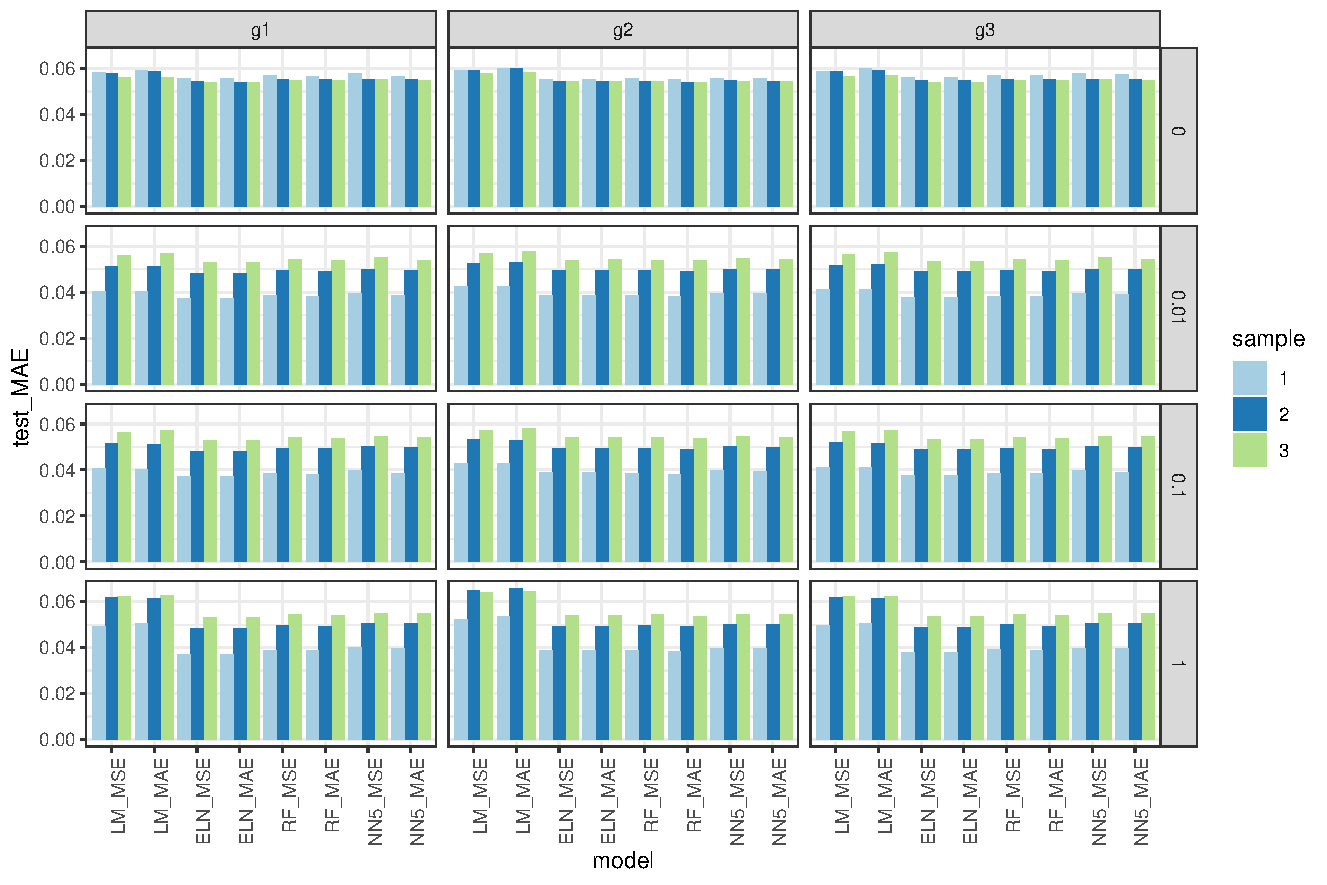
\includegraphics[max size = {\textwidth}{0.5\textheight}]{simulation_test_mae_pre_all.pdf}
	\caption{Simulation Test MAE}
	\floatfoot{Note: faceted by the different data generating processes at the top, and the degree of cross sectional correlation on the right. The y axis represents the MAE on the test set, and the x axis denotes the model (LM = Linear Model, ELN = Elastic Net, RF = Random Forest, NNX = Neural Network with X hidden layers), as well as the loss function it was fitted with respect to. The better performing loss function is bolded for emphasis. Note that only Neural Network 5, the of the neural networks, was shown here.}
	\label{fig:simulation_loss_metrics}
\end{figure}

\begin{figure}[!htb]
	\centering
%	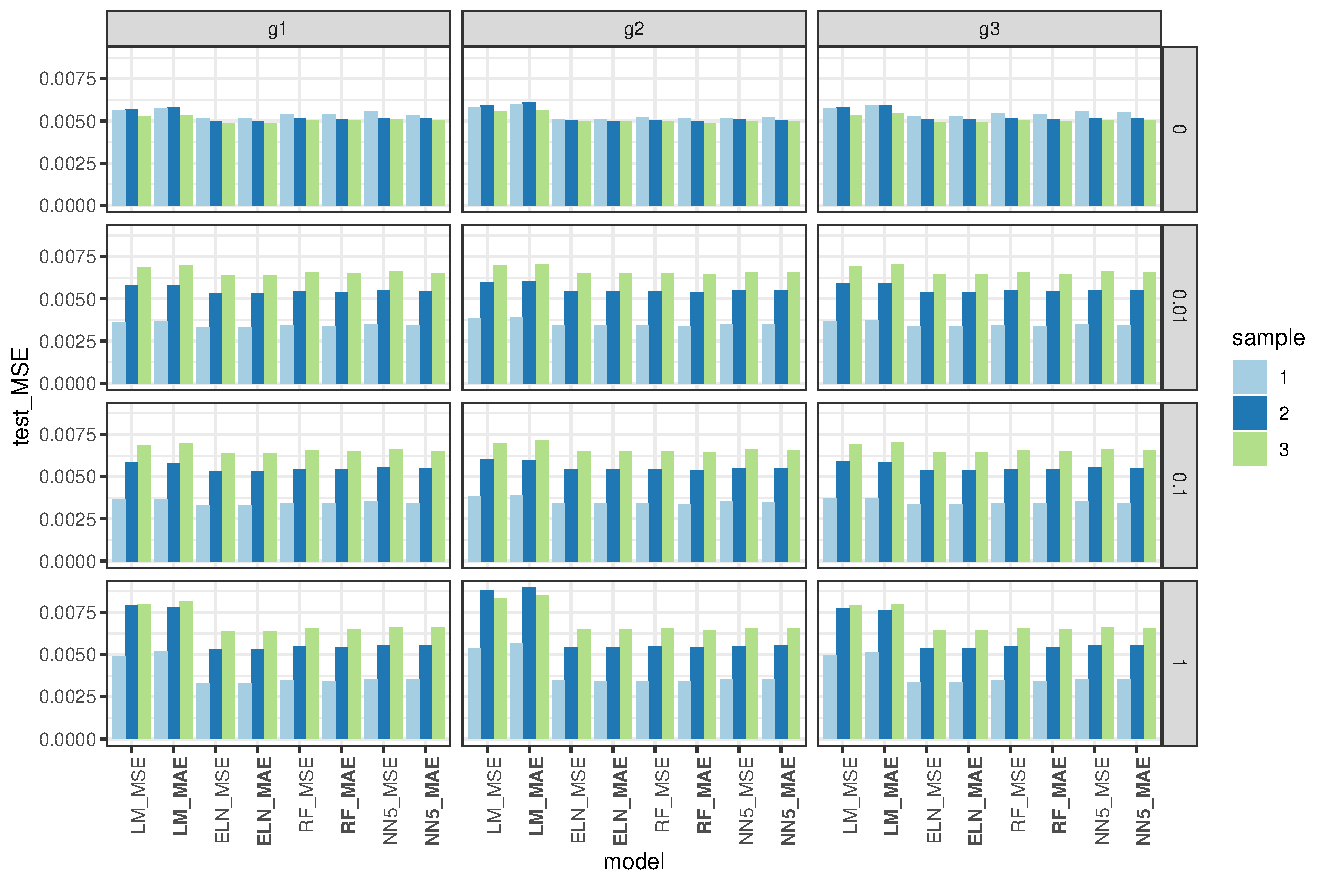
\includegraphics[max size = {\textwidth}{0.5\textheight}]{simulation_test_mse_pre_all.pdf}
	\caption{Simulation Test MSE, see Figure \ref{fig:simulation_loss_metrics} for naming conventions}
\end{figure}

\begin{figure}[!htb]
	\centering
%	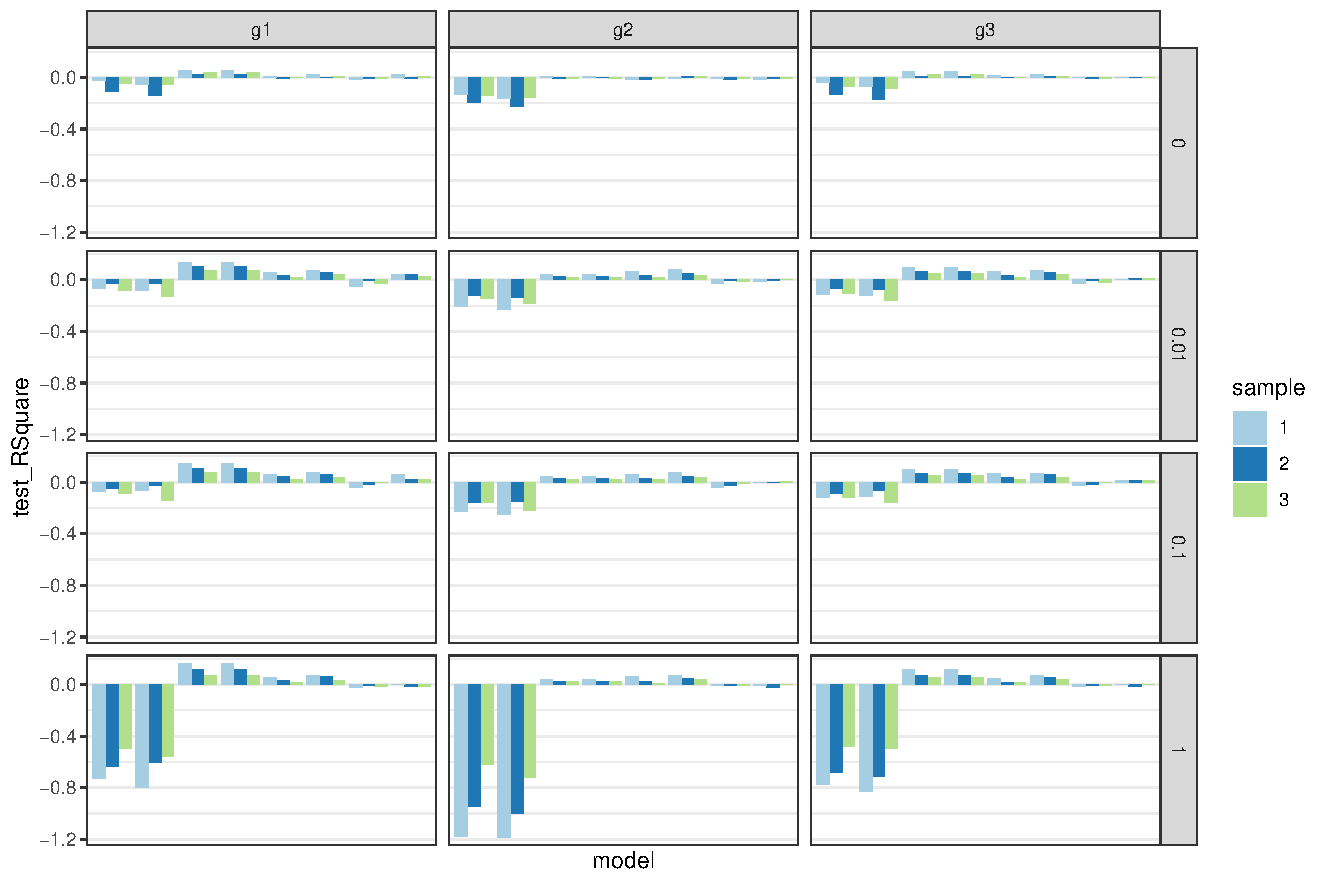
\includegraphics[max size = {\textwidth}{0.5\textheight}]{simulation_test_rsquare_pre_all.pdf}
	\caption{Simulation Test MSE, see Figure \ref{fig:simulation_loss_metrics} for naming conventions}
\end{figure}

Across all specifications with a stochastic volatility component, we observe a decrease in prediction performance as the sample size increased according to the expanding window approach implemented. This is likely due a larger sample having a higher chance to experiences external shocks due to the stochastic volatility process, and thus a higher chance to experience large outliers in the training sample, leading to worse prediction performance. This indicates that machine learning performs poorly when the training data supplied contains more large outliers, and is still sensitive to such outliers even with the use of regularization and robust loss functions.

Focusing on the neural networks, we clearly see that they do not outperform any of the other machine learning models, even when the underlying data generating process is non-linear. This directly contradicts the result which \cite{gu_empirical_2018} find, even when considering the design with no cross sectional correlation and stochastic volatility (top row in graphs), which corresponds to their exact specification but with a multivariate macroeconomic series. We also find consistent evidence that deeper architectures provide better prediction performance, another result which contradicts \cite{gu_empirical_2018}'s conclusions that shallow learning may be better.

\subsubsection{Factor Importance}

Focusing on the factor selection capabilities of different models by looking at variable importance metrics however reveals a more interesting comparison between models. We can clearly observe that the elastic net outperforms all other models consistently in terms of assigning the correct relative importance to the true underlying regressors \footnote{($c_1.\text{constant}$, $c_2.\text{constant}$ and $c_3.x_3$ for $g1$ and $g_2$ specifications, and $c_1.\text{constant}$, $c_2.\text{constant}$ and $c_3.\text{constant}$ for $g_3$)}, even in settings with very high cross sectional correlation. 

In terms of finding the correct underlying regressors, we find that the penalized linear models perform the best at identifying the true data generating regressors, and that this appears to be mostly robust regardless of the amount of cross sectional correlation in the factor set. The penalized linear models are not perfect and their ability to correctly identify underlying regressors worsens as the data generating process becomes more non-linear. On these more difficult specifications, the penalized linear models are generally very conservative, sometimes only identifying a single covariate as important. This is most apparent on the $g_2$ specification. Occasionally, the elastic nets identified the incorrect covariates completely, though the relative importance assigned to them was small. 

The random forests and to a lesser extent the neural networks also correctly identified the correct underlying regressors, but struggled with adequately discerning relative importance among correlated regressors. This was became more apparent as the degree of cross sectional correlation increased (see decreasing relative importance of true underlying regressors in Figures \ref{fig:rf_sim_vi} and \ref{fig:nn_sim_vi} in Appendix). In the case of the random forests, this is to be expected, likely due to how the random forest algorithms work. The random forest algorithm is an ensemble of tree models, with each tree model only having access to a subset of all available predictors. If this subset does not include the true data generating predictor, then that particular tree will likely select the predictors which have the highest correlation with the true data generating predictor instead. Thus, the resulting ensemble model is likely to believe that cross sectionally correlated predictors are important, relative to the true underlying regressor. Due to the complexity of the neural networks, there does not exist a similar intuitive explanation for their factor selection ability.

\begin{landscape}
	\begin{figure}[!htb]
		\begin{center}
	%		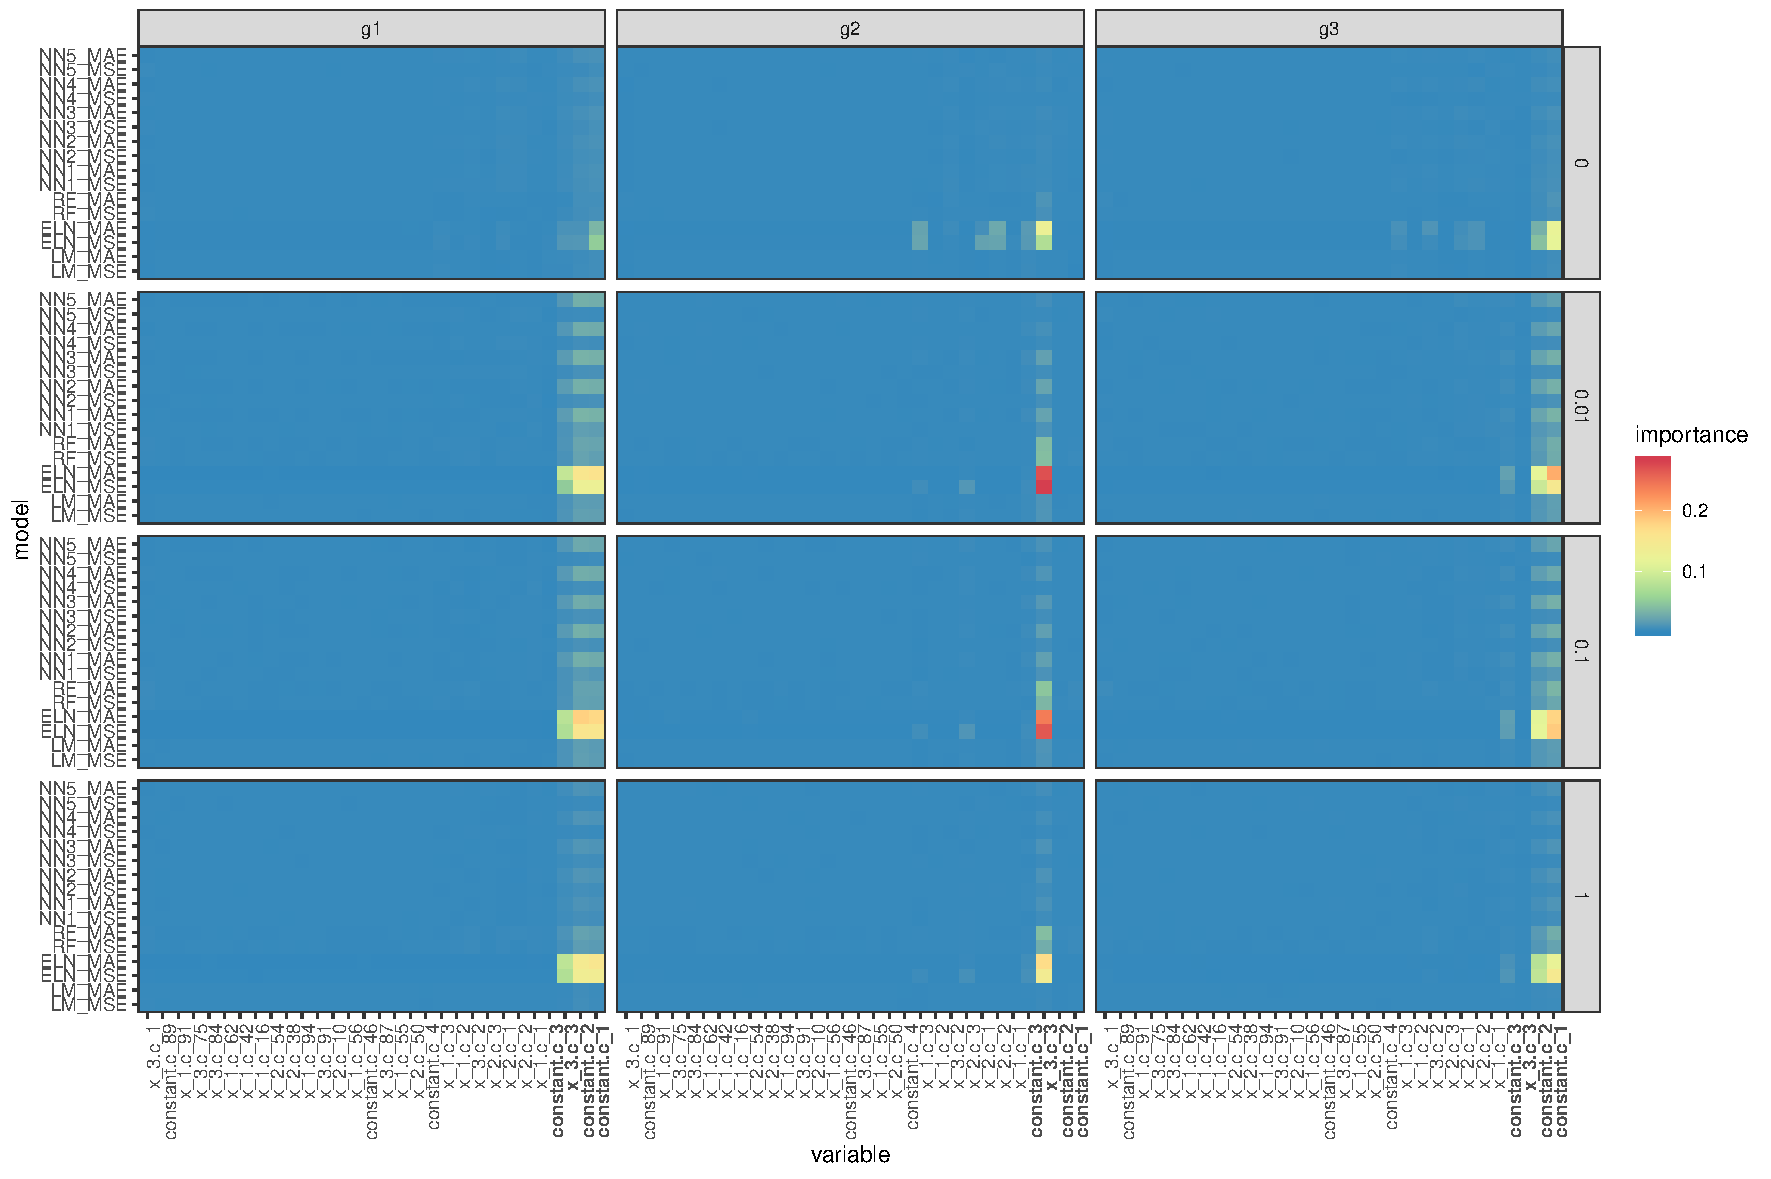
\includegraphics[max size = {23cm}{23cm}]{simulation_ave_vi_plot.pdf}
			\caption{Simulation Variable Importance averaged across all test samples}
			\floatfoot{Note: faceted by data generating specification at the top, and degree of cross-sectional correlation on the right. Model is on the y axis and follows the naming convention in Figure \ref{fig:simulation_loss_metrics}. Factor is on the x axis, and only contains the top 30 important factors, as measured by average importance across all samples and models. Note that the four true underlying factors are bolded.}
		\end{center}
	\end{figure}
\end{landscape}

The linear models, unsurprisingly, struggled with factor significance analysis with respect to both increasing cross sectional correlation and increasing non-linearities. This highlights the non-robustness and ineffectiveness of using traditional linear regression as documented by the literature; linear models were consistently observed to identify irrelevant regressors as important, especially as the degree of cross sectional correlation increased. Considering that the graphs represent the averaged variable importance metrics over different simulation realisations which each have random patterns of cross sectional correlation, this means that on a single simulation realization, the performance of linear models is significantly worse.

%% Brief other notes that are not too important

The overall high performance of the elastic net models may be somewhat surprising given its relative simplicity compared to other machine learning models. However, when recalling that elastic net models are the only machine learning models which are specifically noted to perform well on datasets with high degrees of multicollinearity, the result is perhaps less surprising. Indeed, random forest and neural network models are only noted to be better at capturing non-linear relationships in independent and identically distributed data, a property which we observe on the non-linear specification, and only for the random forests.

Of particular note are the instability of the machine learning models' hyperparameters across different training samples. For the elastic nets, the optimal value for $\alpha$ is generally 1 (corresponding to LASSO and thus a sparse representation), but it was not uncommon to observe $\alpha$ values swinging between values close to 0 (corresponding to ridge regression, and thus a dense representation) to 1 as the training sample moved forwards in time. As the penalized linear models consistently performed the best and still remained able to correctly identify the true covariates this is not a large issue, but it should be noted that this can lead to interpretation issues. For the random forests, it was similarly observed that the optimal value for $mtry$ (the number of variables subsetted) and $nodesize$ was highly non-robust. Again, given that the final prediction performance was consistent this is not a large issue, but can lead to some interpretation issues.


\section{Empirical analysis}

We conduct an empirical study as a final way to corroborate the findings of the properties of machine learning models which we observed in the simulation study. Though our simulation study was aimed at capturing the main features of observed data, the underlying data generating process for empirical returns is unknown. This study thus acts as a robustness check as to how machine learning performs on real world data, which can be significantly more complex and noisy than simulated contexts. Our two studies together can be thought of a repeated sampling exercise in exploring how machine learning methods perform on datasets which feature the ``stylized facts" of empirical returns. This empirical study also acts as a final validation against what has been reported in the literature.

Importantly, we find that our findings from the simulation study are largely corroborated for empirical returns data.

\subsection{Data}

We begin by obtaining monthly individual price data from CRSP for all firms listed in the NYSE, AMEX and NASDAQ, starting from 1957 (starting date of the S\&P 500) and ending in December 2016, totalling 60 years. To build individual factors, we construct a factor set based on the cross section of returns literature. This data was sourced from and is the same data used in \cite{gu_empirical_2018}. Like our initial returns sample, it begins in March 1957 and ends in December 2016, totalling 60 years. It contains 94 stock level characteristics: 61 updated annually, 13 updated quarterly and 20 updated monthly, in addition to 74 industry dummies corresponding the the first two digits of the Standard Industrial Classification (SIC) codes. It is noted that this dataset so far contains all securities traded, including those with a CRSP share code other than 10 or 11 and thus includes instruments such as REITs and mutual funds, and those with a share price of less than \$5.

% Begin Cleaning

We detail our cleaning procedure of this dataset. To reduce the size of the dataset and increase feasibility, the dataset was filtered such that only stocks traded primarily on NASDAQ were included (using the PRIMEXCH variable from WRDS). Then, penny stocks (also referred to as microcaps in the literature) with a stock price of less than \$5 were filtered out, as is commonly done in the literature to reduce variability. Stocks without a share code of 10 or 11 (referring to equities) were filtered out, so that securities that are not equities were not included (such as REITs and trust funds). The dataset is provided in a monthly format, which means that many of the factors which are updated only quarterly or annually have very low levels of variability, which can lead to misleading results in the model fitting process. To achieve a balance between having a dataset with enough data points and variability among factors, the dataset was converted to a quarterly format. Quarterly returns were then constructed using the PRC variable according to actual returns (ie not logged differences):

\begin{equation}
RET_t = \frac{PRC_t - PRC_{t-1}}{PRC_{t-1}}
\end{equation}

We allow all stocks which have a quarterly return to enter the dataset, even if they disappear from the dataset for certain periods, as opposed to only keeping stocks which appear continuously throughout the entire period. This was primarily done to reduce survivorship bias in the dataset, which can be very prevalent in financial data, and also allows for stocks which were unlisted and relisted again to feature in the dataset. This has the obvious drawback of introducing some bias in the dataset, as attrition in the dataset is likely to be non-random and correlated with the stocks' returns. 

The sic2 variable, corresponding to the stocks' Standard Industrial Classification (SIC) codes was also dropped. The SIC code system suffers from inconsistent logic in classifying companies, and as a system built for pre-1970s traditional industries has been slow in recognizing new and emerging industries. Indeed, WRDS explicitly cautions the use of SIC codes beyond the use of rough grouping of industries, warning that SIC codes are not strictly enforced by government agencies for accuracy, in addition to most large companies belonging to multiple SIC codes over time. Because of this latter point in particular, there can be inconsistencies on the correct SIC code for the same company depending on the data source. Dropping the sic2 variable also reduced the dimensionality of the dataset by 74 columns, significant increasing computational feasibility.

There existed a significant amount of missing data in the dataset. The dataset's columns were first examined, and any characteristics that had over 20\% of their data were removed. However, as the amount of missing data increases dramatically going further back in time, a balance between using more periods at the cost of removing more characteristics versus using less periods but keeping more characteristics was needed. 1993 Q3 was determined to be a reasonable time frame to begin the dataset, as there was a noticeable increase in data availability and quality after this time.  Missing characteristics were then imputed using their cross sectional medians for each year. 

We then follow \cite{gu_empirical_2018} and construct eight macroeconomic factors following the variable definitions in \cite{welch_comprehensive_2008}: dividend-price ratio (dp), earnings-price ratio (ep), book-to-market ratio (bm), net equity expansion (ntis), Treasury-bill rate (tbl), term spread (tms), default spread (dfy) and stock variance (svar). These factors were lagged by one period so as to be used to predict one period ahead quarterly returns. The treasury bill rate was also used from this source to proxy for the risk free rate in order to construct excess quarterly returns. 

\begin{table}
	\caption{Macroeconomic Factors, (\cite{welch_comprehensive_2008})}
	\label{macro_factors}
	\begin{center}
		\begin{tabular}{lccc} \hline
			No. & Acronym & Macroeconomic Factor \\ \hline
			1 & macro\_dp & Dividend Price Ratio \\
			2 & macro\_ep & Earnings Price Ratio \\
			3 & macro\_bm & Book to Market Ratio \\
			4 & macro\_ntis & Net Equity Expansion \\
			5 & macro\_tbl & Treasury Bill Rate \\
			6 & macro\_tms & Term Spread \\
			7 & macro\_dfy & Default Spread \\
			8 & macro\_svar & Stock Variance \\ \hline
		\end{tabular}
	\end{center}
\end{table}

The two sets of factors were then combined to form a baseline set of covariates, which we define throughout all methods and analysis as:

\begin{equation}
z_{i,t} = (1, x_t)' \otimes c_{i, t}
\end{equation}

where $c_{i,t}$ is a $P_c$ matrix of characteristics for each stock $i$, and $(1, x_t)'$ is a $P_x \times 1$ vector of macroeconomic predictors, , and $\otimes$ represents the Kronecker product. $z_{i,t}$ is therefore a $P_x P_c$ vector of features for predicting individual stock returns and includes interactions between stock level characteristics and macroeconomic variables. The total number of covariates in this baseline set is $61 \times (8 + 1) = 549$\footnote{As the individual and macroeconomic factors can have similar names, individual and macroeconomic factors were prefixed with ind\_ and macro\_ respectively.}.

% Splitting Scheme
% Similar splitting scheme to simulation study used
% Training:Validation size ratio of 1.5, growing and moving forwards by 1 year
% To maintain feasibility, only 3 samples were conducted

The dataset was not normalized for all methods, as only penalized regression and neural networks are sensitive to normalization. For these two methods, the dataset was normalized such that each predictor column had 0 mean and 1 variance.

The final dataset spanned from 1993 Q3 to 2016 Q4 with 202, 066 individual observations.

We mimic the procedure used in the simulation study. For the sample splitting procedure, the dataset was split such that the training and validation sets were split such that the training set was approximately 1.5 times the length of the validation set, in order to predict a test set that is one year in length.

\begin{figure}[!htb]
	\begin{center}
		\begin{tabular}{|c|p{0.55cm}p{0.55cm}p{0.50cm}p{0.50cm}p{0.50cm}p{0.50cm}p{0.50cm}p{0.50cm}p{0.50cm}p{0.50cm}p{0.50cm}p{0.50cm}p{0.50cm}p{0.50cm}p{0.50cm}p{0.50cm}|}
			\hline
			Set No. &&&&&&&&&&&&&&&& \\
			\hline
			%%%%%%%%
			3 & \cellcolor{cyan} & \cellcolor{cyan} & \cellcolor{cyan} & \cellcolor{cyan} & \cellcolor{cyan} & \cellcolor{cyan} & \cellcolor{cyan} & \cellcolor{cyan} &
			\cellcolor{pink} & \cellcolor{pink} & \cellcolor{pink} & \cellcolor{pink} & \cellcolor{pink} & \cellcolor{pink} & \cellcolor{pink} & \cellcolor{olive} \\
			%%%%%%%%
			2 & \cellcolor{cyan} & \cellcolor{cyan} & \cellcolor{cyan} & \cellcolor{cyan} & \cellcolor{cyan} & \cellcolor{cyan} & \cellcolor{cyan} &
			\cellcolor{pink} & \cellcolor{pink} & \cellcolor{pink} & \cellcolor{pink} & \cellcolor{pink} & \cellcolor{pink} & \cellcolor{pink} & 	
			\cellcolor{olive} & NA \\
			%%%%%%%%
			1 & \cellcolor{cyan} & \cellcolor{cyan} & \cellcolor{cyan} & \cellcolor{cyan} & \cellcolor{cyan} & \cellcolor{cyan} &
			\cellcolor{pink} & \cellcolor{pink} & \cellcolor{pink} & \cellcolor{pink} & \cellcolor{pink} & \cellcolor{pink} & \cellcolor{pink} & \cellcolor{olive} & NA & NA \\
			\hline
			Time & 93Q3 & 93Q4 & 94 & 95 & 96 & ... & 06 & 07 & 08 & ... & 11 & 12 & 13 & 14 & 15 & 16 \\
			\hline
		\end{tabular}
		\medskip
		\begin{tabular}{|c|p{0.60cm}|}
			\hline
			Training & \cellcolor{cyan} \\
			\hline
			Validation & \cellcolor{pink} \\
			\hline
			Test & \cellcolor{olive} \\
			\hline
		\end{tabular}
	\end{center}
	\caption{Empirical Data Sample Splitting Procedure}
	\label{emp_sample_split_diag}
\end{figure}

\newpage

\subsection{Empirical Data Results}

% Overall Results

In general, the empirical results are in remarkable agreement with the those obtained in the simulation study. In particular, we similarly see that the penalized linear models generally performing the best, with the random forest models offering slightly worse performance, occasionally outperforming penalized linear models. Machine learning models fitted with respect to median quantile loss were similarly observed to typically offer improvements across all machine learning models across all loss metrics. 

\subsubsection{Prediction Accuracy}

In terms of prediction accuracy, we can see that in general the results of the simulation study were repeated: the elastic net models perform the best, followed by the random forests, then the neural networks, and finally the linear models. We note that the differences between each model using the MSE and MAE loss metrics are much more pronounced on empirical data. Even so, the predictive performance between the elastic net models and the quantile random forests is not particularly large, and we observe the quantile random forests outperforming the elastic nets in the first data sample. We similarly see that machine learning models perform better when fitted with respect to quantile loss instead of MSE. Most notably, we start to see the neural network models performing poorly on the empirical data, a direct contradiction to what has been reported in the literature.

\begin{figure}[!htb]
	\centering
	%	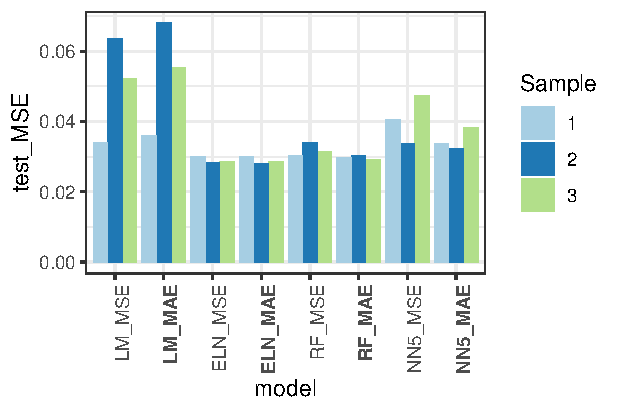
\includegraphics[max size = {\textwidth}{0.4\textheight}]{empirical_test_mse_pre_all}
	\caption{Empirical Test MSE}
	\floatfoot{Note: Test MSE on y axis, with model on x axis, following naming convention in Figure \ref{fig:simulation_loss_metrics}}
\end{figure}

\begin{figure}[!htb]
	\centering
	%	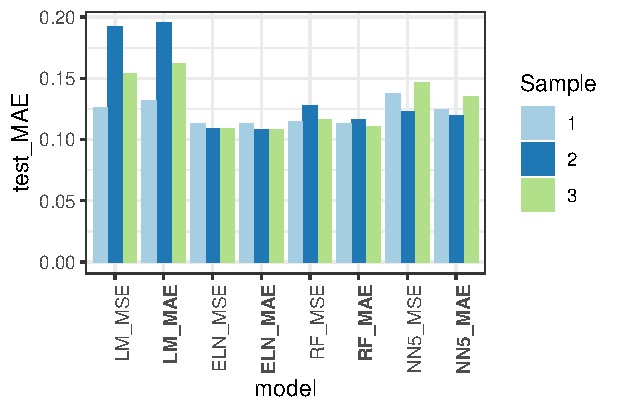
\includegraphics[max size = {\textwidth}{0.4\textheight}]{empirical_test_mae_pre_all}
	\caption{Empirical Test MAE}
	\floatfoot{Note: Test MAE on y axis, with model on x axis, following naming convention in Figure \ref{fig:simulation_loss_metrics}}
\end{figure}

\begin{figure}[!htb]
	\centering
	%	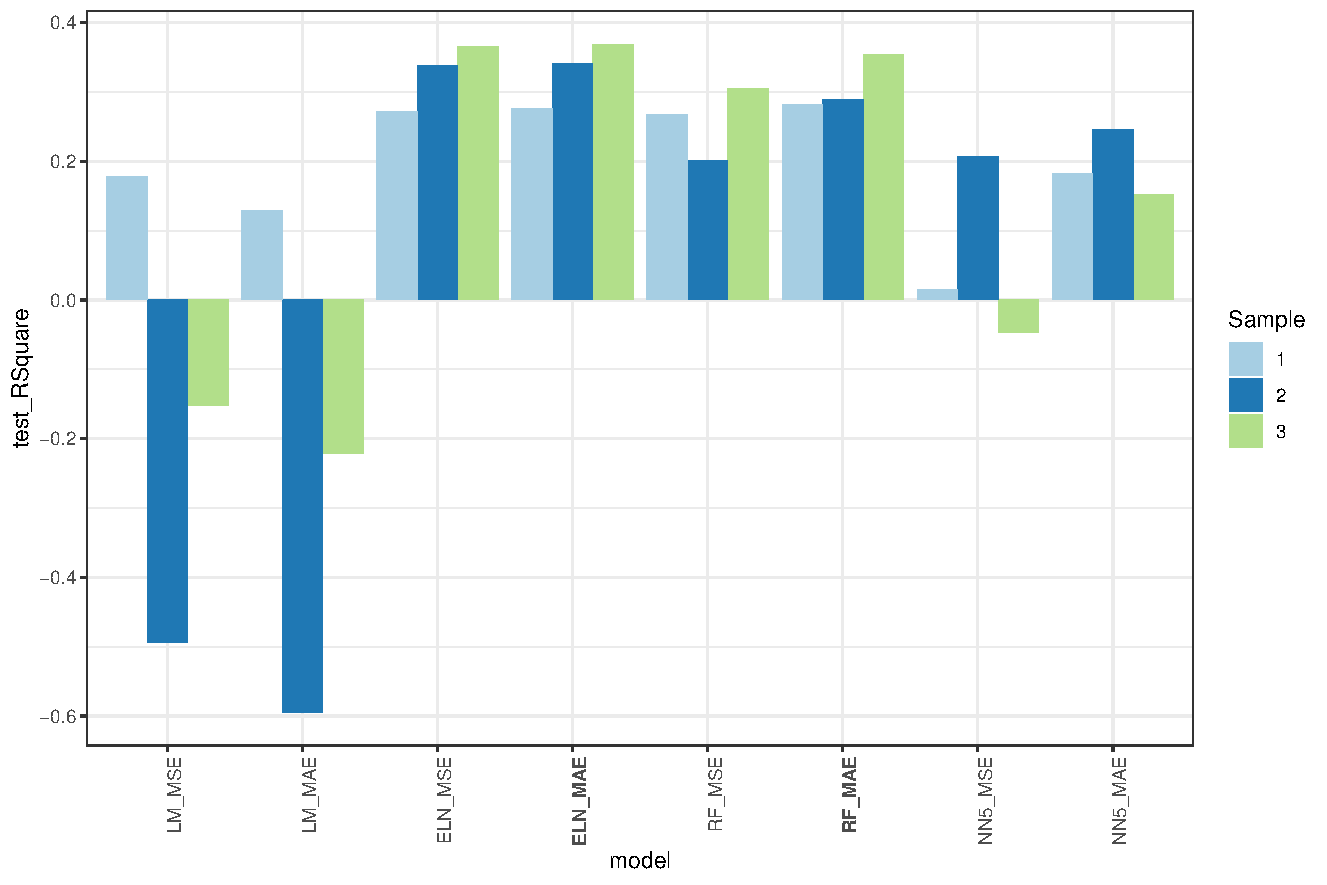
\includegraphics[max size = {\textwidth}{0.4\textheight}]{empirical_test_rsquare_pre_all}
	\caption{Empirical Test Predictive R-Squared}
	\floatfoot{Note: Test Predictive R-Squared on y axis, with model on x axis, following naming convention in Figure \ref{fig:simulation_loss_metrics}}
\end{figure}

Focusing on the neural networks specifically, their non-robustness is amplified on the empirical dataset, with some neural networks in some samples even performing worse than linear models. This was observed to be somewhat more common on neural networks fitted with respect to MSE, suggesting that they are indeed very sensitive to outliers in training data. We similarly observe some evidence that deeper neural networks perform better, though this result is less apparent due to the lower robustness on empirical data (see \ref{empirical_study_appendix} in Appendix for results).

Interestingly, we do not observe worsening performance as the training sample increases as we did in the simulation study. This suggests that the simulation design may have been too volatile when compared to the specific empirical time periods examined.


\subsubsection{Factor Importance}

As the data generating process for empirical returns is unknown, the variable importance results cannot be directly compared with those of the simulation study. Even so, we see similar results: the elastic net and random forest models tend to agree on the same subset of predictors, but the random forest struggles to discern between highly correlated regressors. Similar to the prediction performance results, neural networks perform poorly.

\begin{figure}[!htb]
	\centering
	%	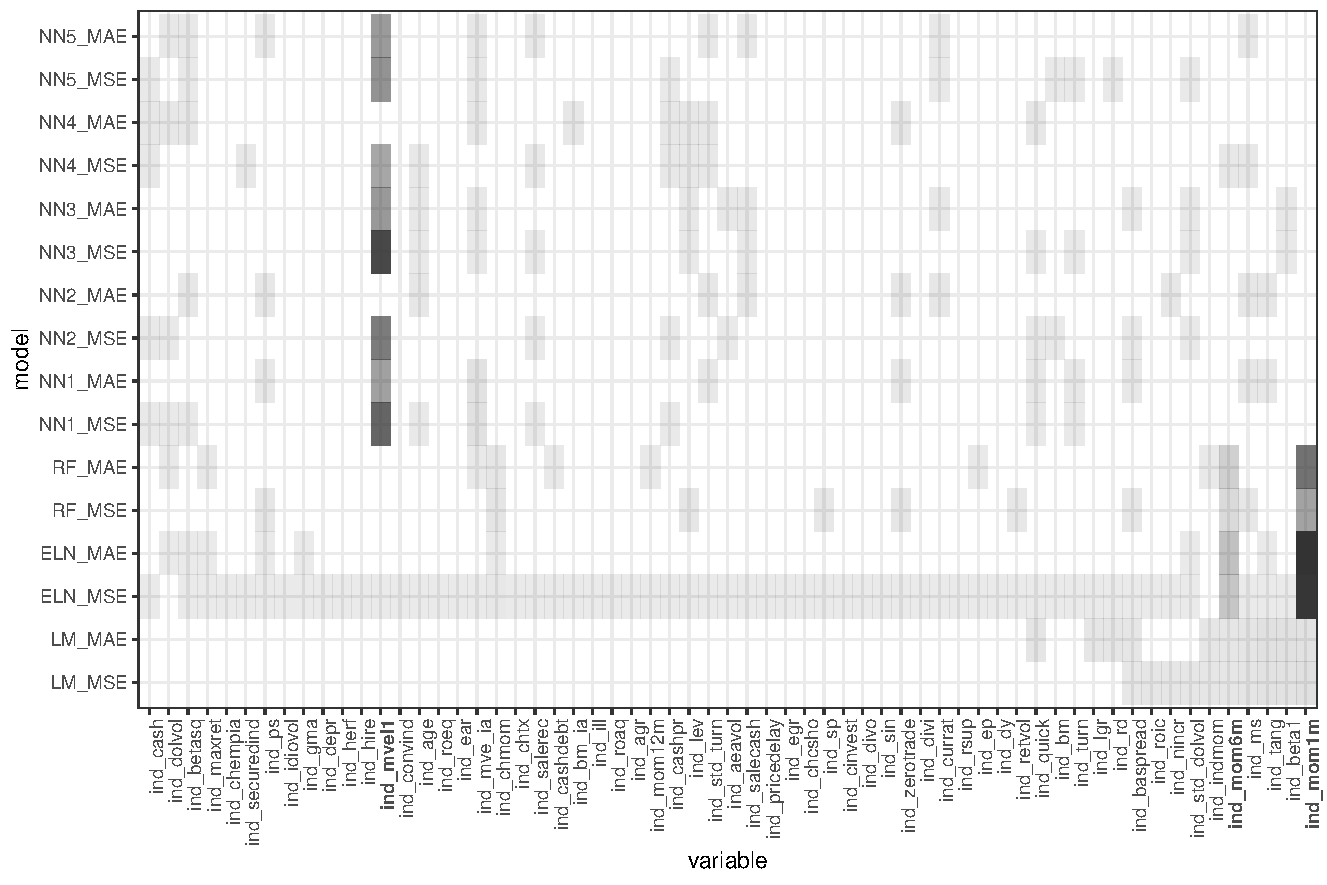
\includegraphics[max size = {\textwidth}{0.35\textheight}]{empirical_sample_all_vi_ind}
	\caption{Empirical Individual Factor Importance, averaged across all training samples}
	\floatfoot{Individual factors shown on x axis, with most important variables bolded (see Table \ref{ind_factors} in Appendix for definitions)}
\end{figure}

\begin{figure}[!htb]
	\label{empirical_macro_facet}
	\centering
	%	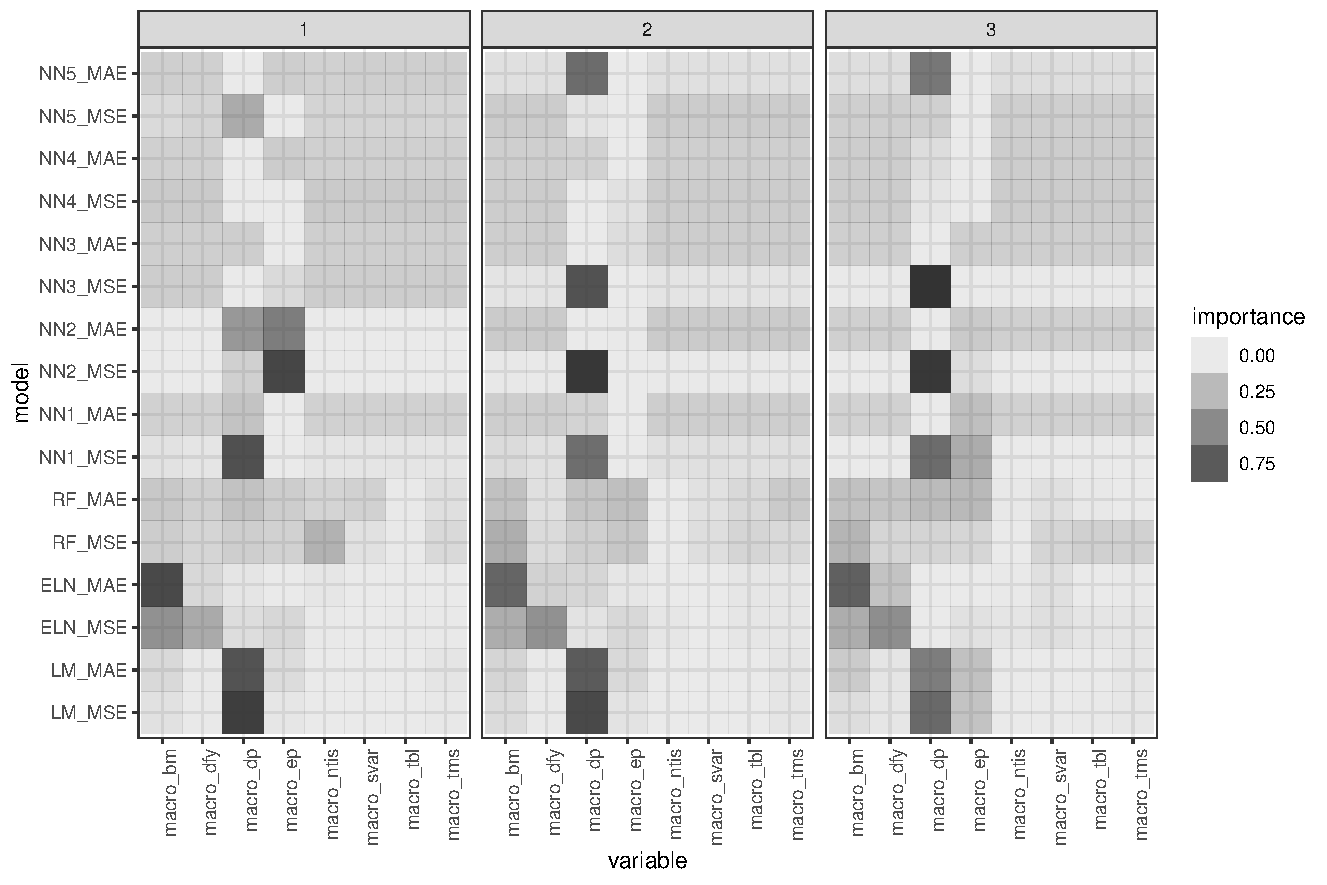
\includegraphics[max size = {\textwidth}{0.35\textheight}]{empirical_sample_all_vi_macro_facet}
	\caption{Empirical Macroeconomic Factor Importance, faceted by training sample}
	\floatfoot{Macroeconomic Factors shown on x axis (see Table \ref{macro_factors} for definitions)}
\end{figure}

If we focus on the two top performing models of elastic net and random forest, we see that they consistently pick out the 1 month and 6 month momentum factors out of the individual characteristics as important, and the book-to-market and default yield spread factors out of the macroeconomic factors are important. In general though, the variable importance metrics are less consistent for the random forests, and it should be noted in particular that the random forest tends to determine factors highly correlated with momentum as important, such as change in moment, dollar trading volume and return volatility. Looking at the macroeconomic factors, penalized linear models tend to identify the average book to market ratio and the default spread as the most important macroeconomic factors. On the macroeconomic factor set, the random forests were inconsistent with the elastic nets, and tended to assign very similar variable importance metrics to most macroeconomic factors.

The neural networks tended to believe that the market value factor was the most important among the individual factors, a result not repeated by any of the other models considered. Within the macroeconomic factors, the neural networks identified and the dividend-price ratio and earnings-price ratio as the most important among the macroeconomic factors, though these results were highly non-robust across different architectures, loss functions and training samples.

Interestingly, we find that the linear models assign the controversial dividend price ratio macroeconomic factor as highly important, a result mirrored only with the neural networks Their variable importance for individual factors across different training samples is highly non-robust, with the important variables almost completely changing year to year. The linear models consistently identified the controversial dividend-price ratio as important, a result that was somewhat consistent with the neural networks. 

The overall results again contradict the results of \cite{gu_empirical_2018}, who conclude that all of the machine methods agree on the same subset of important factors. Indeed, we only see consistency in variable importance between the elastic nets and random forests on the individual factors only - all other variable importance metrics were either inconsistent between different models, or non-robust.

All models considered typically preferred sparse parameterizations. That is, most if not all of the individual factors had little to no importance across all models.\footnote{Note that because the variable importance here was not evaluated explicitly for each pairwise interaction term, some of the individual factors appear as slightly important. This is because setting an individual factor to zero also sets some of the macroeconomic pairwise terms to zero, increasing its apparent importance.}




\section{Conclusion}

Our findings demonstrate that the field of machine learning may offer certain tools to improve stock prediction and identification of true underlying factors. Penalized linear models and to a lesser extent, random forests are the best performing methods in the analysis undertaken.

Importantly, we find that the feed-forward neural network architectures considered by \cite{gu_empirical_2018} fail in the context of stock return prediction, at both prediction performance and variable importance analysis. This result is consistent across a variety of simulated datasets, as well as empirical data. We also find weak evidence that deeper neural networks with more hidden layers perform better, though this result, like the performance of neural networks in general, is non-robust.

Lastly, we find that the top performing models - the penalized linear models and random forests, tend to agree and correctly identify the correct underlying regressors in simulated contexts, as well as agree on the same subset of factors which are important in empirical contexts. We find that of all the most considered, the penalized linear models are the most consistent at identifying true underlying regressors through the simulation study. We find that in the empirical setting, among the individual factors the individual 1 and 6 month momentum factors are the most powerful predictors of stock returns, according to the penalized linear models and random forests. 

Across all models except for linear models, we find that minimizing quantile loss yields better prediction performance.

The overall findings of this paper differ from the sparse literature on machine learning methods in empirical finance. However, the performance of the penalized linear models with respect to both out of sample prediction performance and variable importance analysis is promising, and our findings show that machine learning provides some tools which may aid in the problems of stock return prediction and risk factor selection in the financial world. 

\subsection{Retrieval of style files}

The style files for NeurIPS and other conference information are available on
the World Wide Web at
\begin{center}
  \url{http://www.neurips.cc/}
\end{center}
The file \verb+neurips_2020.pdf+ contains these instructions and illustrates the
various formatting requirements your NeurIPS paper must satisfy.

The only supported style file for NeurIPS 2020 is \verb+neurips_2020.sty+,
rewritten for \LaTeXe{}.  \textbf{Previous style files for \LaTeX{} 2.09,
  Microsoft Word, and RTF are no longer supported!}

The \LaTeX{} style file contains three optional arguments: \verb+final+, which
creates a camera-ready copy, \verb+preprint+, which creates a preprint for
submission to, e.g., arXiv, and \verb+nonatbib+, which will not load the
\verb+natbib+ package for you in case of package clash.

\paragraph{Preprint option}
If you wish to post a preprint of your work online, e.g., on arXiv, using the
NeurIPS style, please use the \verb+preprint+ option. This will create a
nonanonymized version of your work with the text ``Preprint. Work in progress.''
in the footer. This version may be distributed as you see fit. Please \textbf{do
  not} use the \verb+final+ option, which should \textbf{only} be used for
papers accepted to NeurIPS.

At submission time, please omit the \verb+final+ and \verb+preprint+
options. This will anonymize your submission and add line numbers to aid
review. Please do \emph{not} refer to these line numbers in your paper as they
will be removed during generation of camera-ready copies.

The file \verb+neurips_2020.tex+ may be used as a ``shell'' for writing your
paper. All you have to do is replace the author, title, abstract, and text of
the paper with your own.

The formatting instructions contained in these style files are summarized in
Sections \ref{gen_inst}, \ref{headings}, and \ref{others} below.

\section{General formatting instructions}
\label{gen_inst}

The text must be confined within a rectangle 5.5~inches (33~picas) wide and
9~inches (54~picas) long. The left margin is 1.5~inch (9~picas).  Use 10~point
type with a vertical spacing (leading) of 11~points.  Times New Roman is the
preferred typeface throughout, and will be selected for you by default.
Paragraphs are separated by \nicefrac{1}{2}~line space (5.5 points), with no
indentation.

The paper title should be 17~point, initial caps/lower case, bold, centered
between two horizontal rules. The top rule should be 4~points thick and the
bottom rule should be 1~point thick. Allow \nicefrac{1}{4}~inch space above and
below the title to rules. All pages should start at 1~inch (6~picas) from the
top of the page.

For the final version, authors' names are set in boldface, and each name is
centered above the corresponding address. The lead author's name is to be listed
first (left-most), and the co-authors' names (if different address) are set to
follow. If there is only one co-author, list both author and co-author side by
side.

Please pay special attention to the instructions in Section \ref{others}
regarding figures, tables, acknowledgments, and references.

\section{Headings: first level}
\label{headings}

All headings should be lower case (except for first word and proper nouns),
flush left, and bold.

First-level headings should be in 12-point type.

\subsection{Headings: second level}

Second-level headings should be in 10-point type.

\subsubsection{Headings: third level}

Third-level headings should be in 10-point type.

\paragraph{Paragraphs}

There is also a \verb+\paragraph+ command available, which sets the heading in
bold, flush left, and inline with the text, with the heading followed by 1\,em
of space.

\section{Citations, figures, tables, references}
\label{others}

These instructions apply to everyone.

\subsection{Citations within the text}

The \verb+natbib+ package will be loaded for you by default.  Citations may be
author/year or numeric, as long as you maintain internal consistency.  As to the
format of the references themselves, any style is acceptable as long as it is
used consistently.

The documentation for \verb+natbib+ may be found at
\begin{center}
  \url{http://mirrors.ctan.org/macros/latex/contrib/natbib/natnotes.pdf}
\end{center}
Of note is the command \verb+\citet+, which produces citations appropriate for
use in inline text.  For example,
\begin{verbatim}
   \citet{hasselmo} investigated\dots
\end{verbatim}
produces
\begin{quote}
  Hasselmo, et al.\ (1995) investigated\dots
\end{quote}

If you wish to load the \verb+natbib+ package with options, you may add the
following before loading the \verb+neurips_2020+ package:
\begin{verbatim}
   \PassOptionsToPackage{options}{natbib}
\end{verbatim}

If \verb+natbib+ clashes with another package you load, you can add the optional
argument \verb+nonatbib+ when loading the style file:
\begin{verbatim}
   \usepackage[nonatbib]{neurips_2020}
\end{verbatim}

As submission is double blind, refer to your own published work in the third
person. That is, use ``In the previous work of Jones et al.\ [4],'' not ``In our
previous work [4].'' If you cite your other papers that are not widely available
(e.g., a journal paper under review), use anonymous author names in the
citation, e.g., an author of the form ``A.\ Anonymous.''

\subsection{Footnotes}

Footnotes should be used sparingly.  If you do require a footnote, indicate
footnotes with a number\footnote{Sample of the first footnote.} in the
text. Place the footnotes at the bottom of the page on which they appear.
Precede the footnote with a horizontal rule of 2~inches (12~picas).

Note that footnotes are properly typeset \emph{after} punctuation
marks.\footnote{As in this example.}

\subsection{Figures}

\begin{figure}
  \centering
  \fbox{\rule[-.5cm]{0cm}{4cm} \rule[-.5cm]{4cm}{0cm}}
  \caption{Sample figure caption.}
\end{figure}

All artwork must be neat, clean, and legible. Lines should be dark enough for
purposes of reproduction. The figure number and caption always appear after the
figure. Place one line space before the figure caption and one line space after
the figure. The figure caption should be lower case (except for first word and
proper nouns); figures are numbered consecutively.

You may use color figures.  However, it is best for the figure captions and the
paper body to be legible if the paper is printed in either black/white or in
color.

\subsection{Tables}

All tables must be centered, neat, clean and legible.  The table number and
title always appear before the table.  See Table~\ref{sample-table}.

Place one line space before the table title, one line space after the
table title, and one line space after the table. The table title must
be lower case (except for first word and proper nouns); tables are
numbered consecutively.

Note that publication-quality tables \emph{do not contain vertical rules.} We
strongly suggest the use of the \verb+booktabs+ package, which allows for
typesetting high-quality, professional tables:
\begin{center}
  \url{https://www.ctan.org/pkg/booktabs}
\end{center}
This package was used to typeset Table~\ref{sample-table}.

\begin{table}
  \caption{Sample table title}
  \label{sample-table}
  \centering
  \begin{tabular}{lll}
    \toprule
    \multicolumn{2}{c}{Part}                   \\
    \cmidrule(r){1-2}
    Name     & Description     & Size ($\mu$m) \\
    \midrule
    Dendrite & Input terminal  & $\sim$100     \\
    Axon     & Output terminal & $\sim$10      \\
    Soma     & Cell body       & up to $10^6$  \\
    \bottomrule
  \end{tabular}
\end{table}

\section{Final instructions}

Do not change any aspects of the formatting parameters in the style files.  In
particular, do not modify the width or length of the rectangle the text should
fit into, and do not change font sizes (except perhaps in the
\textbf{References} section; see below). Please note that pages should be
numbered.

\section{Preparing PDF files}

Please prepare submission files with paper size ``US Letter,'' and not, for
example, ``A4.''

Fonts were the main cause of problems in the past years. Your PDF file must only
contain Type 1 or Embedded TrueType fonts. Here are a few instructions to
achieve this.

\begin{itemize}

\item You should directly generate PDF files using \verb+pdflatex+.

\item You can check which fonts a PDF files uses.  In Acrobat Reader, select the
  menu Files$>$Document Properties$>$Fonts and select Show All Fonts. You can
  also use the program \verb+pdffonts+ which comes with \verb+xpdf+ and is
  available out-of-the-box on most Linux machines.

\item The IEEE has recommendations for generating PDF files whose fonts are also
  acceptable for NeurIPS. Please see
  \url{http://www.emfield.org/icuwb2010/downloads/IEEE-PDF-SpecV32.pdf}

\item \verb+xfig+ "patterned" shapes are implemented with bitmap fonts.  Use
  "solid" shapes instead.

\item The \verb+\bbold+ package almost always uses bitmap fonts.  You should use
  the equivalent AMS Fonts:
\begin{verbatim}
   \usepackage{amsfonts}
\end{verbatim}
followed by, e.g., \verb+\mathbb{R}+, \verb+\mathbb{N}+, or \verb+\mathbb{C}+
for $\mathbb{R}$, $\mathbb{N}$ or $\mathbb{C}$.  You can also use the following
workaround for reals, natural and complex:
\begin{verbatim}
   \newcommand{\RR}{I\!\!R} %real numbers
   \newcommand{\Nat}{I\!\!N} %natural numbers
   \newcommand{\CC}{I\!\!\!\!C} %complex numbers
\end{verbatim}
Note that \verb+amsfonts+ is automatically loaded by the \verb+amssymb+ package.

\end{itemize}

If your file contains type 3 fonts or non embedded TrueType fonts, we will ask
you to fix it.

\subsection{Margins in \LaTeX{}}

Most of the margin problems come from figures positioned by hand using
\verb+\special+ or other commands. We suggest using the command
\verb+\includegraphics+ from the \verb+graphicx+ package. Always specify the
figure width as a multiple of the line width as in the example below:
\begin{verbatim}
   \usepackage[pdftex]{graphicx} ...
   \includegraphics[width=0.8\linewidth]{myfile.pdf}
\end{verbatim}
See Section 4.4 in the graphics bundle documentation
(\url{http://mirrors.ctan.org/macros/latex/required/graphics/grfguide.pdf})

A number of width problems arise when \LaTeX{} cannot properly hyphenate a
line. Please give LaTeX hyphenation hints using the \verb+\-+ command when
necessary.


\section*{Broader Impact}

Authors are required to include a statement of the broader impact of their work, including its ethical aspects and future societal consequences. 
Authors should discuss both positive and negative outcomes, if any. For instance, authors should discuss a) 
who may benefit from this research, b) who may be put at disadvantage from this research, c) what are the consequences of failure of the system, and d) whether the task/method leverages
biases in the data. If authors believe this is not applicable to them, authors can simply state this.

Use unnumbered first level headings for this section, which should go at the end of the paper. {\bf Note that this section does not count towards the eight pages of content that are allowed.}

\begin{ack}
Use unnumbered first level headings for the acknowledgments. All acknowledgments
go at the end of the paper before the list of references. Moreover, you are required to declare 
funding (financial activities supporting the submitted work) and competing interests (related financial activities outside the submitted work). 
More information about this disclosure can be found at: \url{https://neurips.cc/Conferences/2020/PaperInformation/FundingDisclosure}.


Do {\bf not} include this section in the anonymized submission, only in the final paper. You can use the \texttt{ack} environment provided in the style file to autmoatically hide this section in the anonymized submission.
\end{ack}

\section*{References}

References follow the acknowledgments. Use unnumbered first-level heading for
the references. Any choice of citation style is acceptable as long as you are
consistent. It is permissible to reduce the font size to \verb+small+ (9 point)
when listing the references.
{\bf Note that the Reference section does not count towards the eight pages of content that are allowed.}
\medskip

\small

[1] Alexander, J.A.\ \& Mozer, M.C.\ (1995) Template-based algorithms for
connectionist rule extraction. In G.\ Tesauro, D.S.\ Touretzky and T.K.\ Leen
(eds.), {\it Advances in Neural Information Processing Systems 7},
pp.\ 609--616. Cambridge, MA: MIT Press.

[2] Bower, J.M.\ \& Beeman, D.\ (1995) {\it The Book of GENESIS: Exploring
  Realistic Neural Models with the GEneral NEural SImulation System.}  New York:
TELOS/Springer--Verlag.

[3] Hasselmo, M.E., Schnell, E.\ \& Barkai, E.\ (1995) Dynamics of learning and
recall at excitatory recurrent synapses and cholinergic modulation in rat
hippocampal region CA3. {\it Journal of Neuroscience} {\bf 15}(7):5249-5262.


\appendix


\section{Additional details: dimulation design}
In this section, we give additional features of the simulation design required to implenent our results. All code and data can be found at XXXX. 

\subsection{Simulation Design}

We begin with the simulation study as a way to explore how machine learning performs with specific regards to the characteristics present in financial data. By specifying a simulation design with the desired characteristics, a controlled and well understood environment is available for explicitly testing the predictive performance and factor selection capabilities of the machine learning models considered. In particular, a simulation design which incorporated the following characteristics of financial data was needed:

\begin{itemize}
	\item Low signal to noise ratio
	\item Stochastic volatility in errors (including large random external shocks and volatility clustering)
	\item Persistence in regressors
	\item Cross sectional correlation (multicollinearity) in regressors
\end{itemize}

\subsubsection{Overall Design}

We first construct our simulation design by considering the design considered by \cite{gu_empirical_2018}, which consists of three overall components:
\begin{itemize}
	\item Simulate individual firm and macroeconomic factors
	\item Enter these factors into a latent, true data generating process
	\item Produce the overall returns process as this latent generative process plus an error process
\end{itemize}

However, \cite{gu_empirical_2018}'s specification has two main issues: the factors which enter the return equation are uncorrelated across each stock $i$, and the error process specified amounts to a white noise, constant volatility specification. As noted by \cite{harvey__2016} and many others, this is not what is observed in practice. 

We therefore simulate a latent factor model with a stochastic volatility process for excess returns  $r_{t+1}$, for $t=1,\dots,T$:

\begin{align}
r_{i, t+1} &= 
g\left(z_{i, t}\right) + \beta_{i,t+1}v_{t+1} + e_{i, t+1}; 
\quad z_{i, t}=\left(1, x_{t}\right)^{\prime} \otimes c_{i, t}, 
\quad \beta_{i, t}=\left(c_{i 1, t}, c_{i 2, t}, c_{i 3, t}\right) \\ 
e_{i, t+1} &= 
\sigma_{i, t+1} \varepsilon_{i, t+1}; \\
\operatorname{log} (\sigma^2_{i,t+1}) &= 
\omega + \gamma \operatorname{log} (\sigma^2_{t}) + \sigma_{u}u; 
\quad u \sim N(0, 1)
\end{align}

Let $v_{t+1}$ be a $3\times 1$ vector of errors, and $w_{t+1} \sim N(0, 1)$ and $\varepsilon_{i,t+1} \sim N(0, 1)$ scalar error terms. 

The matrix $C_t$ is an $N\times P_c$ matrix of latent factors, where the first three columns correspond to $\beta_{i,t}$, across the $1\leq i\leq N$ dimensions, while the remaining $P_c-3$ factors do not enter the return equation. The $P_x\times1$ vector $x_t$ is a $3 \times 1$ multivariate time series, and $\varepsilon_{t+1}$ is a $N\times 1$ vector of idiosyncratic errors. 

The parameters of these were tuned such that the annualized volatility of each return series was approximately 22\%, as is often observed empirically.

Note that we also reproduce \cite{gu_empirical_2018}'s error specification as a case where there is no stochastic volatility:

\begin{align}
v_{t+1} \sim N(0, 0.05^2 \times I_3) \\
e_{i, t+1} \sim t_5(0, 0.05^2)
\end{align}

\subsubsection{Simulating Characteristics}

A simulation mechanism for $C_t$ that gives some correlation across the factors and across time was used. We build in correlation across time among factors by drawing normal random numbers for each $1\leq i\leq N$ and $1\leq j\leq P_{c}$, according to 

\begin{equation}
\overline{c}_{i j, t} = \rho_{j} \overline{c}_{i j, t-1}+\epsilon_{i j, t} ;
\quad \rho_{j} \sim \mathcal{U} \left( \frac{1}{2},1 \right) 
\end{equation}

To build in cross sectional correlation, we define the positive-semidefinite matrix $B$:

\begin{equation}
B:=\Lambda\Lambda' + \frac{1}{10}\mathbb{I}_{n}, \quad
\Lambda_i = (\lambda_{i1},\dots,\lambda_{i4}), \quad
\lambda_{ik}\sim N(0, \lambda_{sd}), \; k=1, \dots, 4
\end{equation}

to serve as a variance covariance matrix with $\lambda_{sd}$ controlling the density of the matrix, and hence degree of cross sectional correlation. $\lambda_{sd}$ values of 0.01, 0.1 and 1 were used to explore increasing degrees of cross sectional correlation.

To build this into our $N\times P_{c}$ characteristics matrix $\bar{C}_t$, we simulate characteristics according to

\begin{equation}
\widehat{C}_{t}=L\overline{C}_{t} ; \quad B = LL' 
\end{equation}

where $L$ represents the lower triangle matrix of $B$ using the Cholesky decomposition.

Finally, the "observed" characteristics for each $1\leq i\leq N$ and for $j=1, \dots, P_{c}$ are constructed according to:

\begin{equation}
c_{i j, t} = \frac{2}{n+1} \operatorname{rank}\left(\hat{c}_{i j, t}\right) - 1.
\end{equation}

with the rank transformation normalizing all predictors to be within $[-1, 1]$. 

\subsubsection{Simulating Macroeconomic Series}

For simulation of $x_{t}$, a $3 \times 1$ multivariate time series, we consider a Vector Autoregression (VAR) model \footnote{Other more complex and interactive matrix specifications of $A$ were briefly explored, but these did not appear to have a significant impact on results. More complex designs were observed to only affect the variable importance metrics, but to an insignificant degree}:

\begin{flalign*}
x_{t} = Ax_{t-1}+u_t; 
\quad A = 
\begin{pmatrix}
.95 & 0 & 0 \\
0 & .95 & 0 \\
0 & 0 & .95
\end{pmatrix} \;
\quad u_t \sim N\left( \mu = (0, 0, 0)' , \Sigma = I_3
\right) 
\end{flalign*}

\subsubsection{Simulating Return Series}

We consider three different functions for $g(z_{i, t})$:

\begin{align}
(1)\; & g_1 \left(z_{i, t}\right)=\left(c_{i 1, t}, c_{i 2, t}, c_{i 3, t} \times x_{t}'[3,]\right) \theta_{0} \\
(2)\; & g_2 \left(z_{i, t}\right)=\left(c_{i 1, t}^{2}, c_{i 1, t} \times c_{i 2, t}, \operatorname{sgn}\left(c_{i 3, t} \times  x_{t}'[3,]\right)\right) \theta_{0} \\
(3)\; & g_3 \left(z_{i, t}\right) = \left(1[c_{i3,t}>0],c_{i 2, t}^{3}, c_{i 1, t} \times c_{i 2, t}\times 1[c_{i3,t}>0], \text{logit}\left({c}_{i3, t} \right)\right) \theta_{0}
\end{align}

where $x_{t}'[3,]$ denotes the third element of the $x_{t}'$ vector.

$g_1 \left(z_{i, t}\right)$ allows the characteristics to enter the return equation linearly, and $g_2 \left(z_{i, t}\right)$ allows the characteristics to enter the return equation interactively and non-linearly. The true underlying regressors for these specifications are $\left(c_{i 1, t}, c_{i 2, t}, c_{i 3, t} \times x_{t}'[3,]\right)$.These two specifications correspond to the simulation design used by \cite{gu_empirical_2018}. 

$g_3 \left(z_{i, t}\right)$ allows the characteristics to enter in a complex and non-linear fashion. The true underlying regressors for this specification are $\left(c_{i 1, t}, c_{i 2, t}, c_{i 3, t} \right)$. 

It should be noted however, that because $g_2 \left(z_{i, t}\right)$ has a large part of its signal entering through a $\operatorname{sgn}$ function, this should make it the most difficult to estimate given the regressors and resulting returns process.

$\theta^0$ was tuned such that the predictive $R^2$ was approximately 5\%.

The simulation design results in $3 \times 3 = 12$ different simulated datasets, each with $N = 200$ stocks, $T = 180$ periods and $P_c = 100$ characteristics. Each design was simulated 10 times to assess the robustness of machine learning algorithms. The number of simulations was kept low for computational feasibility.

\subsubsection{Sample Splitting}

If viewed as monthly periods, $T = 180$ corresponds to 15 years. A data splitting scheme similar to the scheme to be used in the empirical data study was used: a training:validation length ratio of approximately 1.5 to begin, and a test set that is 1 year in length. We employ the hybrid growing window approach as described earlier in section \ref{sample_split} (see Figure \ref{sample_split_diag} for a graphical representation).

\begin{figure}[!htb]
	\begin{center}
		\begin{tabular}{|c|p{0.40cm}p{0.40cm}p{0.40cm}p{0.40cm}p{0.40cm}p{0.40cm}p{0.40cm}p{0.40cm}p{0.40cm}p{0.40cm}p{0.40cm}p{0.40cm}p{0.40cm}p{0.40cm}p{0.40cm}|}
			\hline
			Set No. &&&&&&&&&&&&&&& \\
			\hline
			%%%%%%%%
			3 & \cellcolor{cyan} & \cellcolor{cyan} & \cellcolor{cyan} & \cellcolor{cyan} & \cellcolor{cyan} & \cellcolor{cyan} & \cellcolor{cyan} & \cellcolor{cyan} & \cellcolor{cyan} &
			\cellcolor{pink} & \cellcolor{pink} & \cellcolor{pink} & \cellcolor{pink} & \cellcolor{pink} & 	
			\cellcolor{olive} \\
			%%%%%%%%
			2 & \cellcolor{cyan} & \cellcolor{cyan} & \cellcolor{cyan} & \cellcolor{cyan} & \cellcolor{cyan} & \cellcolor{cyan} & \cellcolor{cyan} & \cellcolor{cyan} &
			\cellcolor{pink} & \cellcolor{pink} & \cellcolor{pink} & \cellcolor{pink} & \cellcolor{pink} & 	
			\cellcolor{olive} & NA  \\
			%%%%%%%%
			1 & \cellcolor{cyan} & \cellcolor{cyan} & \cellcolor{cyan} & \cellcolor{cyan} & \cellcolor{cyan} & \cellcolor{cyan} & \cellcolor{cyan} &
			\cellcolor{pink} & \cellcolor{pink} & \cellcolor{pink} & \cellcolor{pink} & \cellcolor{pink} & 	
			\cellcolor{olive} & NA & NA \\
			\hline
			Year & 1 & 2 & 3 & 4 & 5 & 6 & 7 & 8 & 9 & 10 & 11 & 12 & 13 & 14 & 15\\
			\hline
		\end{tabular}
		\medskip
		\begin{tabular}{|c|p{0.40cm}|}
			\hline
			Training & \cellcolor{cyan} \\
			\hline
			Validation & \cellcolor{pink} \\
			\hline
			Test & \cellcolor{olive} \\
			\hline
		\end{tabular}
	\end{center}
	\caption{Sample Splitting Procedure}
	\label{sample_split_diag}
\end{figure}

Other schemes in the forecasting literature such as using an ``inner" rolling window validation loop to find the best hyperparameters on average, finally aggregating them in an ``outer" loop for a more robust error were considered but not implemented for a variety of reasons. Firstly, many of the models were computationally too intensive for this to be feasible. More importantly, during the model fitting process it was observed that the optimal hyperparameters for the different rolling windows were highly unstable (see Appendix). Thus, this would have made the selection of the best hyperparameters on average across all windows significantly less meaningful.

%%%%%%%%%%%%%%%%%%%%%%%%%%%%%%%%%%%%%%%%%%%%%%%%%%%%%%%%%%%%%%%%%%%%%%%%%%%%%%%%%%%%%%%%%%%%%%%%%%%%%%%%%%%%%%%%%%
\subsection{Simulation Study Results}

Overall, in the simulation study we observe that in general elastic nets are the best performing model, followed closely by random forests, then neural networks. All machine learning models were unaffected by cross sectional correlation in terms of prediction performance, and had better performance when fitted with respect to quantile loss, in stark contrast to linear models. The random forest only outperformed the elastic nets on highly non-linear specifications. The neural network models were not observed to outperform any of the machine learning models. We note that most of these results contradict the sparse literature, and in particular, the results reported by \cite{gu_empirical_2018}, even on their proposed simulation design.

\subsubsection{Prediction Performance}

Looking at the prediction performance of different models, we find that in general, penalized linear models performed the best, followed extremely closely by random forests and then neural networks, which all outperform the baseline linear models. Most importantly, we observes that for machine learning models, cross sectional correlation does not seem to affect prediction performance by much. This is in stark contrast to the linear models, whose prediction performance is severely affected by both non-linearities, and increasing cross sectional correlation. This result is consistent across all loss metrics, and is most obvious when looking at the out-of-sample R-squared metrics.

Machine learning models fitted with respect to minimizing MAE (quantile loss) generally perform better, even when evaluated against MSE loss metrics. This is not a surprising result, especially considering the stochastic error design which introduces significant shocks to the returns process, leading to large outliers which the mean squared error metric is more sensitive to. Though the actual difference between the loss metrics between the penalized linear models, random forests and neural networks are very small, when considering the consistency of the results across numerous Monte Carlo simulations, the differences in prediction performance, though small, is robust and significant.

\begin{figure}[!htb]
	\centering
%	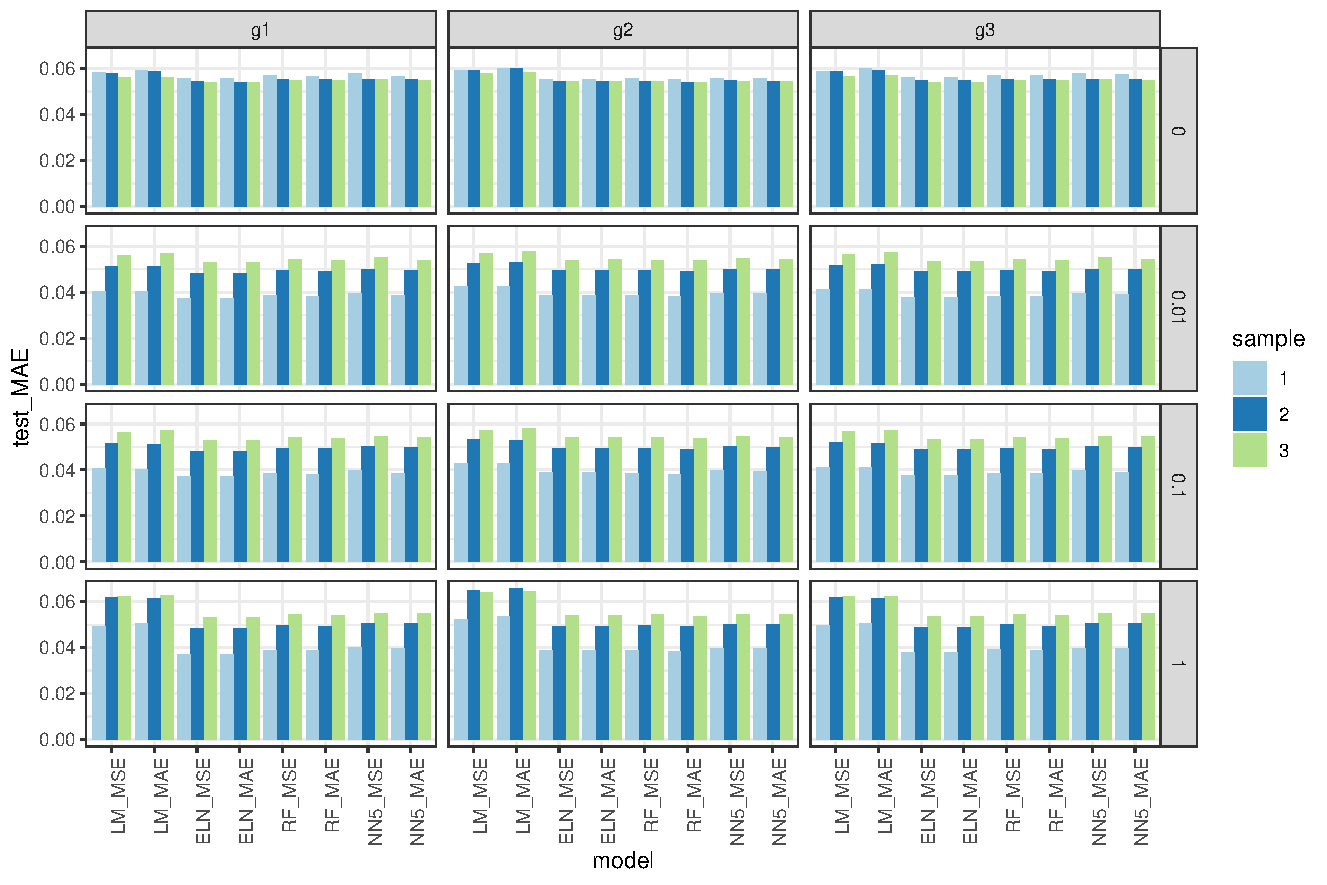
\includegraphics[max size = {\textwidth}{0.5\textheight}]{simulation_test_mae_pre_all.pdf}
	\caption{Simulation Test MAE}
	\floatfoot{Note: faceted by the different data generating processes at the top, and the degree of cross sectional correlation on the right. The y axis represents the MAE on the test set, and the x axis denotes the model (LM = Linear Model, ELN = Elastic Net, RF = Random Forest, NNX = Neural Network with X hidden layers), as well as the loss function it was fitted with respect to. The better performing loss function is bolded for emphasis. Note that only Neural Network 5, the of the neural networks, was shown here.}
	\label{fig:simulation_loss_metrics}
\end{figure}

\begin{figure}[!htb]
	\centering
%	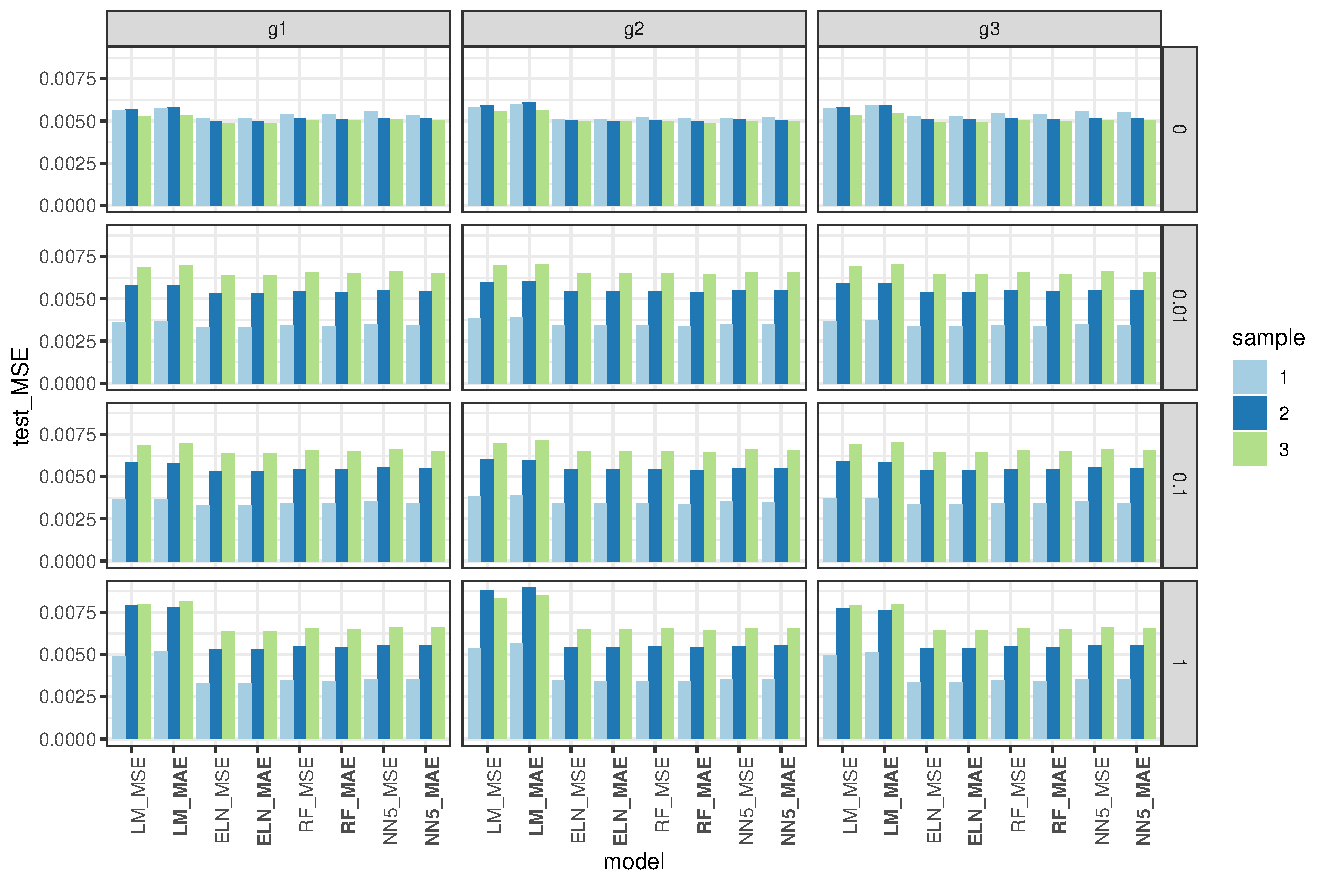
\includegraphics[max size = {\textwidth}{0.5\textheight}]{simulation_test_mse_pre_all.pdf}
	\caption{Simulation Test MSE, see Figure \ref{fig:simulation_loss_metrics} for naming conventions}
\end{figure}

\begin{figure}[!htb]
	\centering
%	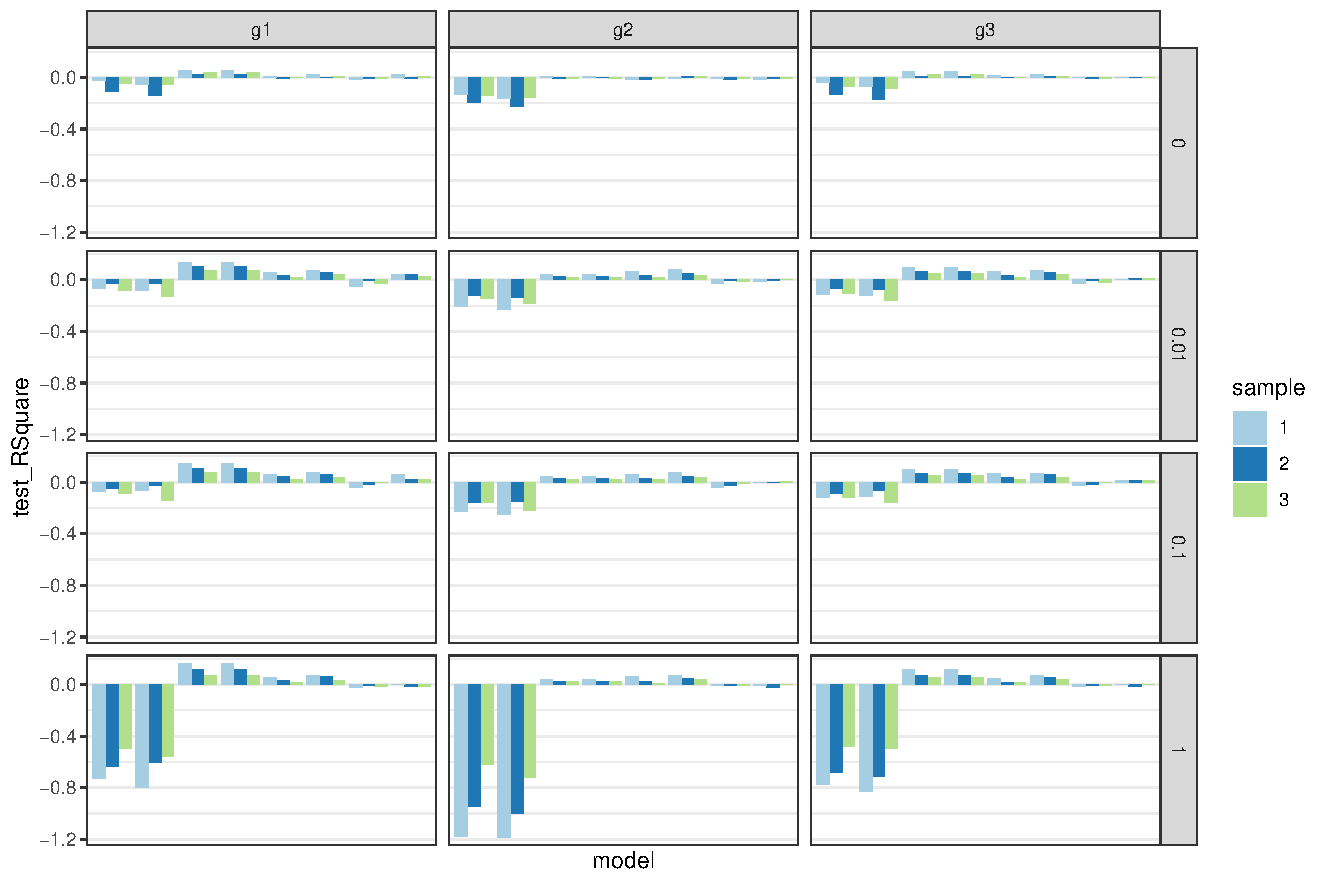
\includegraphics[max size = {\textwidth}{0.5\textheight}]{simulation_test_rsquare_pre_all.pdf}
	\caption{Simulation Test MSE, see Figure \ref{fig:simulation_loss_metrics} for naming conventions}
\end{figure}

Across all specifications with a stochastic volatility component, we observe a decrease in prediction performance as the sample size increased according to the expanding window approach implemented. This is likely due a larger sample having a higher chance to experiences external shocks due to the stochastic volatility process, and thus a higher chance to experience large outliers in the training sample, leading to worse prediction performance. This indicates that machine learning performs poorly when the training data supplied contains more large outliers, and is still sensitive to such outliers even with the use of regularization and robust loss functions.

Focusing on the neural networks, we clearly see that they do not outperform any of the other machine learning models, even when the underlying data generating process is non-linear. This directly contradicts the result which \cite{gu_empirical_2018} find, even when considering the design with no cross sectional correlation and stochastic volatility (top row in graphs), which corresponds to their exact specification but with a multivariate macroeconomic series. We also find consistent evidence that deeper architectures provide better prediction performance, another result which contradicts \cite{gu_empirical_2018}'s conclusions that shallow learning may be better.

\subsubsection{Factor Importance}

Focusing on the factor selection capabilities of different models by looking at variable importance metrics however reveals a more interesting comparison between models. We can clearly observe that the elastic net outperforms all other models consistently in terms of assigning the correct relative importance to the true underlying regressors \footnote{($c_1.\text{constant}$, $c_2.\text{constant}$ and $c_3.x_3$ for $g1$ and $g_2$ specifications, and $c_1.\text{constant}$, $c_2.\text{constant}$ and $c_3.\text{constant}$ for $g_3$)}, even in settings with very high cross sectional correlation. 

In terms of finding the correct underlying regressors, we find that the penalized linear models perform the best at identifying the true data generating regressors, and that this appears to be mostly robust regardless of the amount of cross sectional correlation in the factor set. The penalized linear models are not perfect and their ability to correctly identify underlying regressors worsens as the data generating process becomes more non-linear. On these more difficult specifications, the penalized linear models are generally very conservative, sometimes only identifying a single covariate as important. This is most apparent on the $g_2$ specification. Occasionally, the elastic nets identified the incorrect covariates completely, though the relative importance assigned to them was small. 

The random forests and to a lesser extent the neural networks also correctly identified the correct underlying regressors, but struggled with adequately discerning relative importance among correlated regressors. This was became more apparent as the degree of cross sectional correlation increased (see decreasing relative importance of true underlying regressors in Figures \ref{fig:rf_sim_vi} and \ref{fig:nn_sim_vi} in Appendix). In the case of the random forests, this is to be expected, likely due to how the random forest algorithms work. The random forest algorithm is an ensemble of tree models, with each tree model only having access to a subset of all available predictors. If this subset does not include the true data generating predictor, then that particular tree will likely select the predictors which have the highest correlation with the true data generating predictor instead. Thus, the resulting ensemble model is likely to believe that cross sectionally correlated predictors are important, relative to the true underlying regressor. Due to the complexity of the neural networks, there does not exist a similar intuitive explanation for their factor selection ability.

\begin{landscape}
	\begin{figure}[!htb]
		\begin{center}
	%		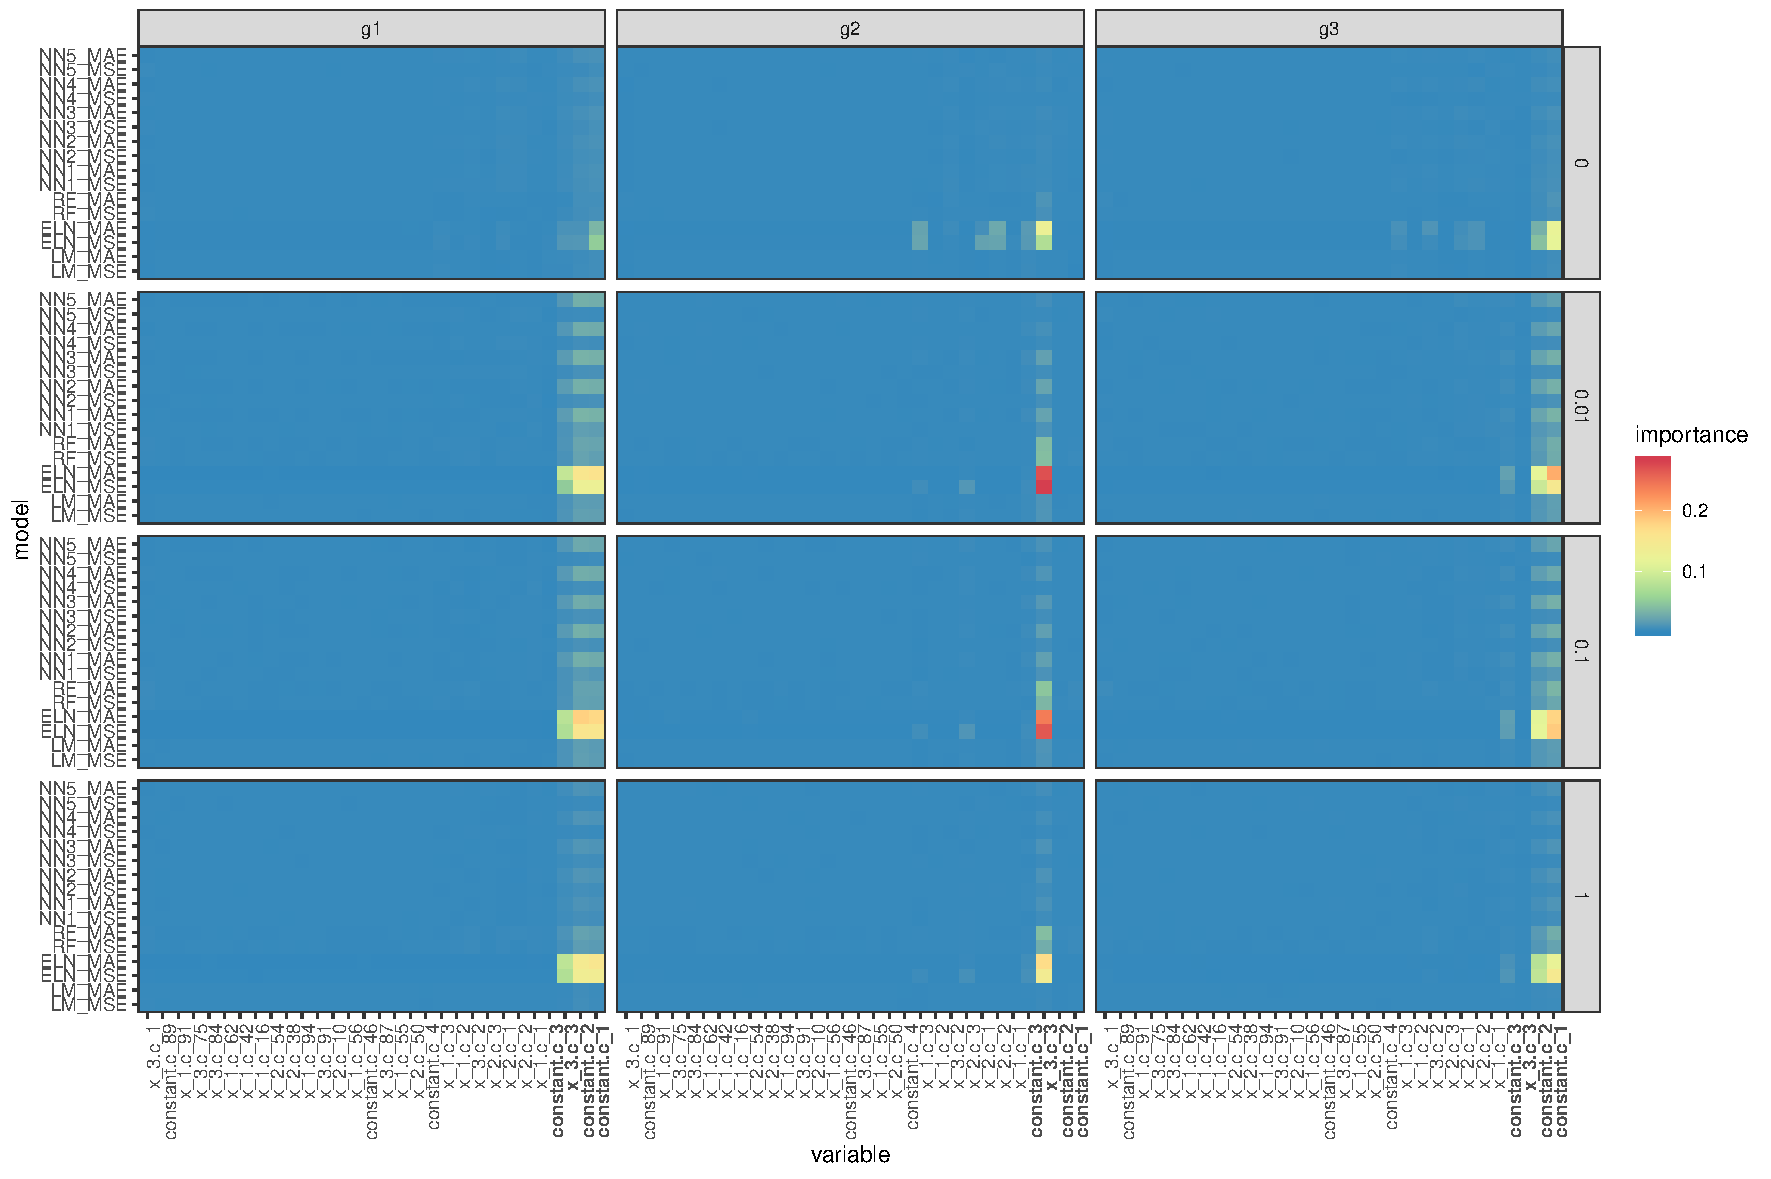
\includegraphics[max size = {23cm}{23cm}]{simulation_ave_vi_plot.pdf}
			\caption{Simulation Variable Importance averaged across all test samples}
			\floatfoot{Note: faceted by data generating specification at the top, and degree of cross-sectional correlation on the right. Model is on the y axis and follows the naming convention in Figure \ref{fig:simulation_loss_metrics}. Factor is on the x axis, and only contains the top 30 important factors, as measured by average importance across all samples and models. Note that the four true underlying factors are bolded.}
		\end{center}
	\end{figure}
\end{landscape}

The linear models, unsurprisingly, struggled with factor significance analysis with respect to both increasing cross sectional correlation and increasing non-linearities. This highlights the non-robustness and ineffectiveness of using traditional linear regression as documented by the literature; linear models were consistently observed to identify irrelevant regressors as important, especially as the degree of cross sectional correlation increased. Considering that the graphs represent the averaged variable importance metrics over different simulation realisations which each have random patterns of cross sectional correlation, this means that on a single simulation realization, the performance of linear models is significantly worse.

%% Brief other notes that are not too important

The overall high performance of the elastic net models may be somewhat surprising given its relative simplicity compared to other machine learning models. However, when recalling that elastic net models are the only machine learning models which are specifically noted to perform well on datasets with high degrees of multicollinearity, the result is perhaps less surprising. Indeed, random forest and neural network models are only noted to be better at capturing non-linear relationships in independent and identically distributed data, a property which we observe on the non-linear specification, and only for the random forests.

Of particular note are the instability of the machine learning models' hyperparameters across different training samples. For the elastic nets, the optimal value for $\alpha$ is generally 1 (corresponding to LASSO and thus a sparse representation), but it was not uncommon to observe $\alpha$ values swinging between values close to 0 (corresponding to ridge regression, and thus a dense representation) to 1 as the training sample moved forwards in time. As the penalized linear models consistently performed the best and still remained able to correctly identify the true covariates this is not a large issue, but it should be noted that this can lead to interpretation issues. For the random forests, it was similarly observed that the optimal value for $mtry$ (the number of variables subsetted) and $nodesize$ was highly non-robust. Again, given that the final prediction performance was consistent this is not a large issue, but can lead to some interpretation issues.

\appendix

\section{Additional details: Empirical analysis}

We conduct an empirical study as a final way to corroborate the findings of the properties of machine learning models which we observed in the simulation study. Though our simulation study was aimed at capturing the main features of observed data, the underlying data generating process for empirical returns is unknown. This study thus acts as a robustness check as to how machine learning performs on real world data, which can be significantly more complex and noisy than simulated contexts. Our two studies together can be thought of a repeated sampling exercise in exploring how machine learning methods perform on datasets which feature the ``stylized facts" of empirical returns. This empirical study also acts as a final validation against what has been reported in the literature.

Importantly, we find that our findings from the simulation study are largely corroborated for empirical returns data.

\subsection{Data}

We begin by obtaining monthly individual price data from CRSP for all firms listed in the NYSE, AMEX and NASDAQ, starting from 1957 (starting date of the S\&P 500) and ending in December 2016, totalling 60 years. To build individual factors, we construct a factor set based on the cross section of returns literature. This data was sourced from and is the same data used in \cite{gu_empirical_2018}. Like our initial returns sample, it begins in March 1957 and ends in December 2016, totalling 60 years. It contains 94 stock level characteristics: 61 updated annually, 13 updated quarterly and 20 updated monthly, in addition to 74 industry dummies corresponding the the first two digits of the Standard Industrial Classification (SIC) codes. It is noted that this dataset so far contains all securities traded, including those with a CRSP share code other than 10 or 11 and thus includes instruments such as REITs and mutual funds, and those with a share price of less than \$5.

% Begin Cleaning

We detail our cleaning procedure of this dataset. To reduce the size of the dataset and increase feasibility, the dataset was filtered such that only stocks traded primarily on NASDAQ were included (using the PRIMEXCH variable from WRDS). Then, penny stocks (also referred to as microcaps in the literature) with a stock price of less than \$5 were filtered out, as is commonly done in the literature to reduce variability. Stocks without a share code of 10 or 11 (referring to equities) were filtered out, so that securities that are not equities were not included (such as REITs and trust funds). The dataset is provided in a monthly format, which means that many of the factors which are updated only quarterly or annually have very low levels of variability, which can lead to misleading results in the model fitting process. To achieve a balance between having a dataset with enough data points and variability among factors, the dataset was converted to a quarterly format. Quarterly returns were then constructed using the PRC variable according to actual returns (ie not logged differences):

\begin{equation}
RET_t = \frac{PRC_t - PRC_{t-1}}{PRC_{t-1}}
\end{equation}

We allow all stocks which have a quarterly return to enter the dataset, even if they disappear from the dataset for certain periods, as opposed to only keeping stocks which appear continuously throughout the entire period. This was primarily done to reduce survivorship bias in the dataset, which can be very prevalent in financial data, and also allows for stocks which were unlisted and relisted again to feature in the dataset. This has the obvious drawback of introducing some bias in the dataset, as attrition in the dataset is likely to be non-random and correlated with the stocks' returns. 

The sic2 variable, corresponding to the stocks' Standard Industrial Classification (SIC) codes was also dropped. The SIC code system suffers from inconsistent logic in classifying companies, and as a system built for pre-1970s traditional industries has been slow in recognizing new and emerging industries. Indeed, WRDS explicitly cautions the use of SIC codes beyond the use of rough grouping of industries, warning that SIC codes are not strictly enforced by government agencies for accuracy, in addition to most large companies belonging to multiple SIC codes over time. Because of this latter point in particular, there can be inconsistencies on the correct SIC code for the same company depending on the data source. Dropping the sic2 variable also reduced the dimensionality of the dataset by 74 columns, significant increasing computational feasibility.

There existed a significant amount of missing data in the dataset. The dataset's columns were first examined, and any characteristics that had over 20\% of their data were removed. However, as the amount of missing data increases dramatically going further back in time, a balance between using more periods at the cost of removing more characteristics versus using less periods but keeping more characteristics was needed. 1993 Q3 was determined to be a reasonable time frame to begin the dataset, as there was a noticeable increase in data availability and quality after this time.  Missing characteristics were then imputed using their cross sectional medians for each year. 

We then follow \cite{gu_empirical_2018} and construct eight macroeconomic factors following the variable definitions in \cite{welch_comprehensive_2008}: dividend-price ratio (dp), earnings-price ratio (ep), book-to-market ratio (bm), net equity expansion (ntis), Treasury-bill rate (tbl), term spread (tms), default spread (dfy) and stock variance (svar). These factors were lagged by one period so as to be used to predict one period ahead quarterly returns. The treasury bill rate was also used from this source to proxy for the risk free rate in order to construct excess quarterly returns. 

\begin{table}
	\caption{Macroeconomic Factors, (\cite{welch_comprehensive_2008})}
	\label{macro_factors}
	\begin{center}
		\begin{tabular}{lccc} \hline
			No. & Acronym & Macroeconomic Factor \\ \hline
			1 & macro\_dp & Dividend Price Ratio \\
			2 & macro\_ep & Earnings Price Ratio \\
			3 & macro\_bm & Book to Market Ratio \\
			4 & macro\_ntis & Net Equity Expansion \\
			5 & macro\_tbl & Treasury Bill Rate \\
			6 & macro\_tms & Term Spread \\
			7 & macro\_dfy & Default Spread \\
			8 & macro\_svar & Stock Variance \\ \hline
		\end{tabular}
	\end{center}
\end{table}

The two sets of factors were then combined to form a baseline set of covariates, which we define throughout all methods and analysis as:

\begin{equation}
z_{i,t} = (1, x_t)' \otimes c_{i, t}
\end{equation}

where $c_{i,t}$ is a $P_c$ matrix of characteristics for each stock $i$, and $(1, x_t)'$ is a $P_x \times 1$ vector of macroeconomic predictors, , and $\otimes$ represents the Kronecker product. $z_{i,t}$ is therefore a $P_x P_c$ vector of features for predicting individual stock returns and includes interactions between stock level characteristics and macroeconomic variables. The total number of covariates in this baseline set is $61 \times (8 + 1) = 549$\footnote{As the individual and macroeconomic factors can have similar names, individual and macroeconomic factors were prefixed with ind\_ and macro\_ respectively.}.

% Splitting Scheme
% Similar splitting scheme to simulation study used
% Training:Validation size ratio of 1.5, growing and moving forwards by 1 year
% To maintain feasibility, only 3 samples were conducted

The dataset was not normalized for all methods, as only penalized regression and neural networks are sensitive to normalization. For these two methods, the dataset was normalized such that each predictor column had 0 mean and 1 variance.

The final dataset spanned from 1993 Q3 to 2016 Q4 with 202, 066 individual observations.

We mimic the procedure used in the simulation study. For the sample splitting procedure, the dataset was split such that the training and validation sets were split such that the training set was approximately 1.5 times the length of the validation set, in order to predict a test set that is one year in length.

\begin{figure}[!htb]
	\begin{center}
		\begin{tabular}{|c|p{0.55cm}p{0.55cm}p{0.50cm}p{0.50cm}p{0.50cm}p{0.50cm}p{0.50cm}p{0.50cm}p{0.50cm}p{0.50cm}p{0.50cm}p{0.50cm}p{0.50cm}p{0.50cm}p{0.50cm}p{0.50cm}|}
			\hline
			Set No. &&&&&&&&&&&&&&&& \\
			\hline
			%%%%%%%%
			3 & \cellcolor{cyan} & \cellcolor{cyan} & \cellcolor{cyan} & \cellcolor{cyan} & \cellcolor{cyan} & \cellcolor{cyan} & \cellcolor{cyan} & \cellcolor{cyan} &
			\cellcolor{pink} & \cellcolor{pink} & \cellcolor{pink} & \cellcolor{pink} & \cellcolor{pink} & \cellcolor{pink} & \cellcolor{pink} & \cellcolor{olive} \\
			%%%%%%%%
			2 & \cellcolor{cyan} & \cellcolor{cyan} & \cellcolor{cyan} & \cellcolor{cyan} & \cellcolor{cyan} & \cellcolor{cyan} & \cellcolor{cyan} &
			\cellcolor{pink} & \cellcolor{pink} & \cellcolor{pink} & \cellcolor{pink} & \cellcolor{pink} & \cellcolor{pink} & \cellcolor{pink} & 	
			\cellcolor{olive} & NA \\
			%%%%%%%%
			1 & \cellcolor{cyan} & \cellcolor{cyan} & \cellcolor{cyan} & \cellcolor{cyan} & \cellcolor{cyan} & \cellcolor{cyan} &
			\cellcolor{pink} & \cellcolor{pink} & \cellcolor{pink} & \cellcolor{pink} & \cellcolor{pink} & \cellcolor{pink} & \cellcolor{pink} & \cellcolor{olive} & NA & NA \\
			\hline
			Time & 93Q3 & 93Q4 & 94 & 95 & 96 & ... & 06 & 07 & 08 & ... & 11 & 12 & 13 & 14 & 15 & 16 \\
			\hline
		\end{tabular}
		\medskip
		\begin{tabular}{|c|p{0.60cm}|}
			\hline
			Training & \cellcolor{cyan} \\
			\hline
			Validation & \cellcolor{pink} \\
			\hline
			Test & \cellcolor{olive} \\
			\hline
		\end{tabular}
	\end{center}
	\caption{Empirical Data Sample Splitting Procedure}
	\label{emp_sample_split_diag}
\end{figure}

\newpage

\subsection{Empirical Data Results}

% Overall Results

In general, the empirical results are in remarkable agreement with the those obtained in the simulation study. In particular, we similarly see that the penalized linear models generally performing the best, with the random forest models offering slightly worse performance, occasionally outperforming penalized linear models. Machine learning models fitted with respect to median quantile loss were similarly observed to typically offer improvements across all machine learning models across all loss metrics. 

\subsubsection{Prediction Accuracy}

In terms of prediction accuracy, we can see that in general the results of the simulation study were repeated: the elastic net models perform the best, followed by the random forests, then the neural networks, and finally the linear models. We note that the differences between each model using the MSE and MAE loss metrics are much more pronounced on empirical data. Even so, the predictive performance between the elastic net models and the quantile random forests is not particularly large, and we observe the quantile random forests outperforming the elastic nets in the first data sample. We similarly see that machine learning models perform better when fitted with respect to quantile loss instead of MSE. Most notably, we start to see the neural network models performing poorly on the empirical data, a direct contradiction to what has been reported in the literature.

\begin{figure}[!htb]
	\centering
%	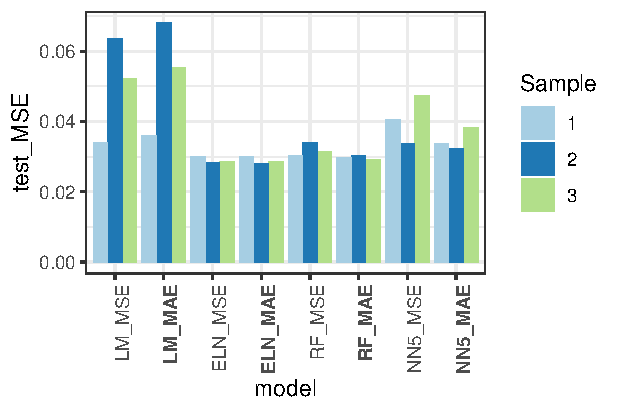
\includegraphics[max size = {\textwidth}{0.4\textheight}]{empirical_test_mse_pre_all}
	\caption{Empirical Test MSE}
	\floatfoot{Note: Test MSE on y axis, with model on x axis, following naming convention in Figure \ref{fig:simulation_loss_metrics}}
\end{figure}

\begin{figure}[!htb]
	\centering
%	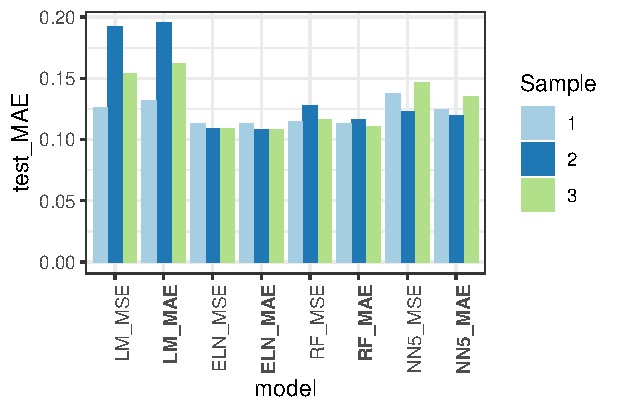
\includegraphics[max size = {\textwidth}{0.4\textheight}]{empirical_test_mae_pre_all}
	\caption{Empirical Test MAE}
	\floatfoot{Note: Test MAE on y axis, with model on x axis, following naming convention in Figure \ref{fig:simulation_loss_metrics}}
\end{figure}

\begin{figure}[!htb]
	\centering
%	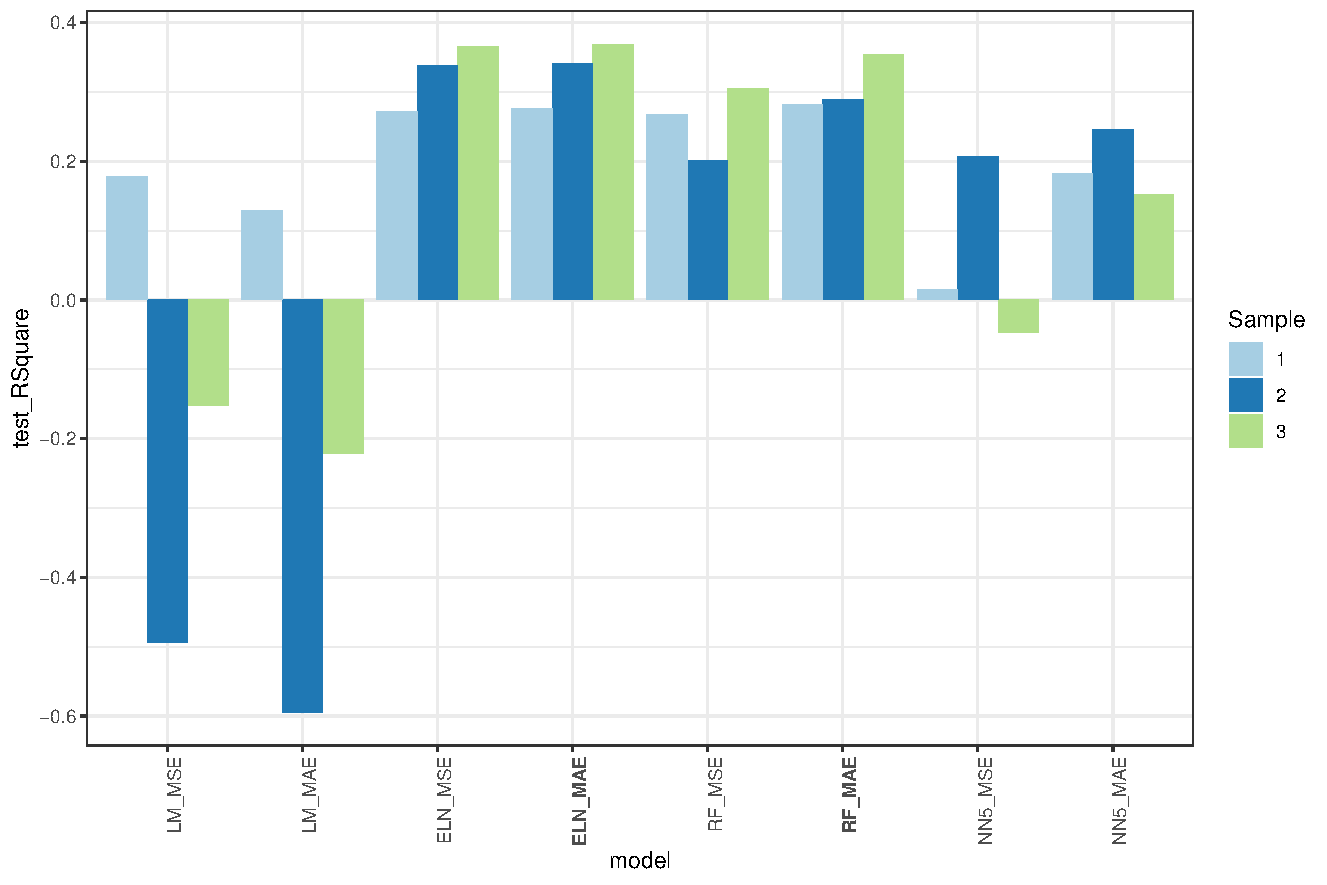
\includegraphics[max size = {\textwidth}{0.4\textheight}]{empirical_test_rsquare_pre_all}
	\caption{Empirical Test Predictive R-Squared}
	\floatfoot{Note: Test Predictive R-Squared on y axis, with model on x axis, following naming convention in Figure \ref{fig:simulation_loss_metrics}}
\end{figure}

Focusing on the neural networks specifically, their non-robustness is amplified on the empirical dataset, with some neural networks in some samples even performing worse than linear models. This was observed to be somewhat more common on neural networks fitted with respect to MSE, suggesting that they are indeed very sensitive to outliers in training data. We similarly observe some evidence that deeper neural networks perform better, though this result is less apparent due to the lower robustness on empirical data (see \ref{empirical_study_appendix} in Appendix for results).

Interestingly, we do not observe worsening performance as the training sample increases as we did in the simulation study. This suggests that the simulation design may have been too volatile when compared to the specific empirical time periods examined.


\subsubsection{Factor Importance}

As the data generating process for empirical returns is unknown, the variable importance results cannot be directly compared with those of the simulation study. Even so, we see similar results: the elastic net and random forest models tend to agree on the same subset of predictors, but the random forest struggles to discern between highly correlated regressors. Similar to the prediction performance results, neural networks perform poorly.

\begin{figure}[!htb]
	\centering
%	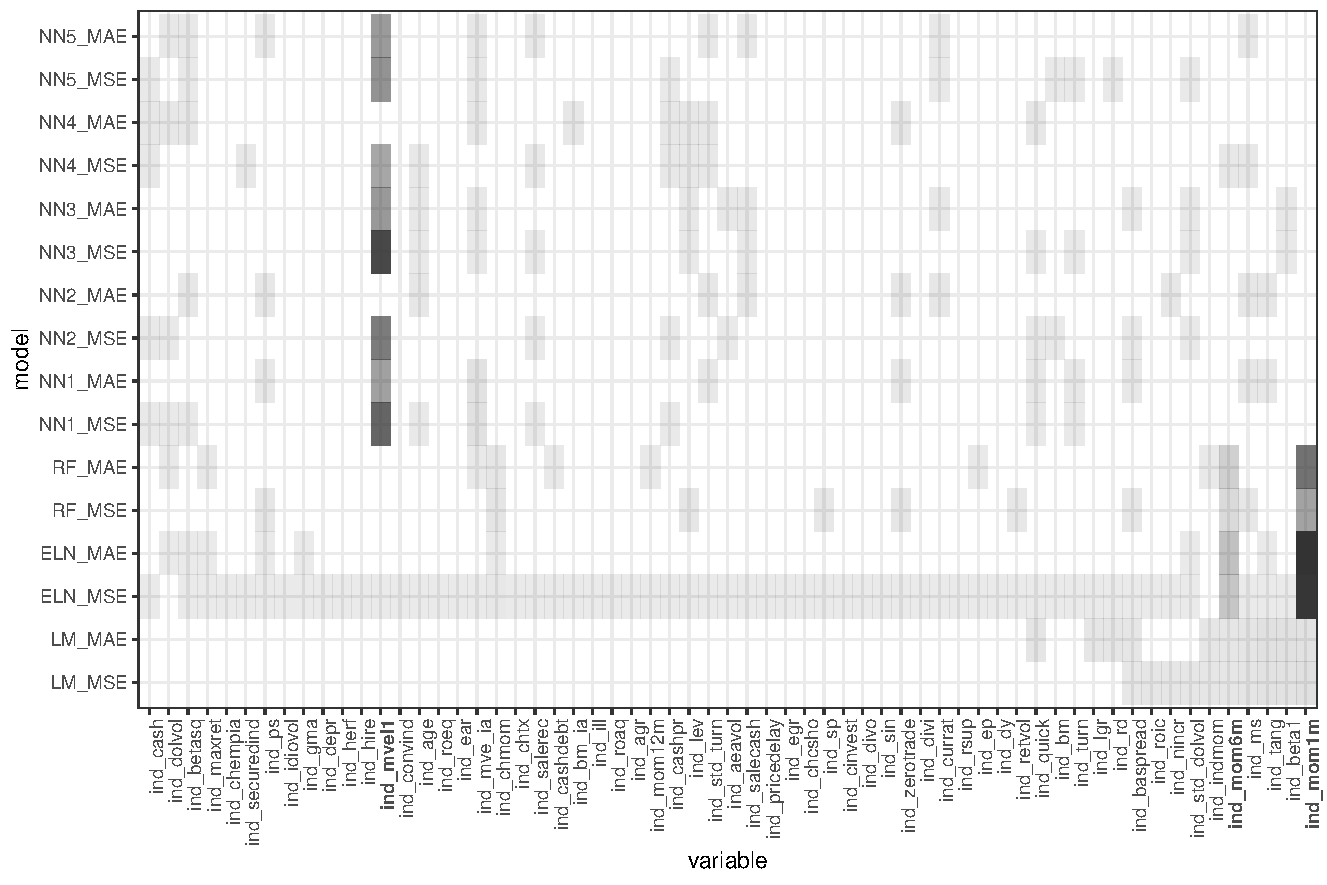
\includegraphics[max size = {\textwidth}{0.35\textheight}]{empirical_sample_all_vi_ind}
	\caption{Empirical Individual Factor Importance, averaged across all training samples}
	\floatfoot{Individual factors shown on x axis, with most important variables bolded (see Table \ref{ind_factors} in Appendix for definitions)}
\end{figure}

\begin{figure}[!htb]
	\label{empirical_macro_facet}
	\centering
%	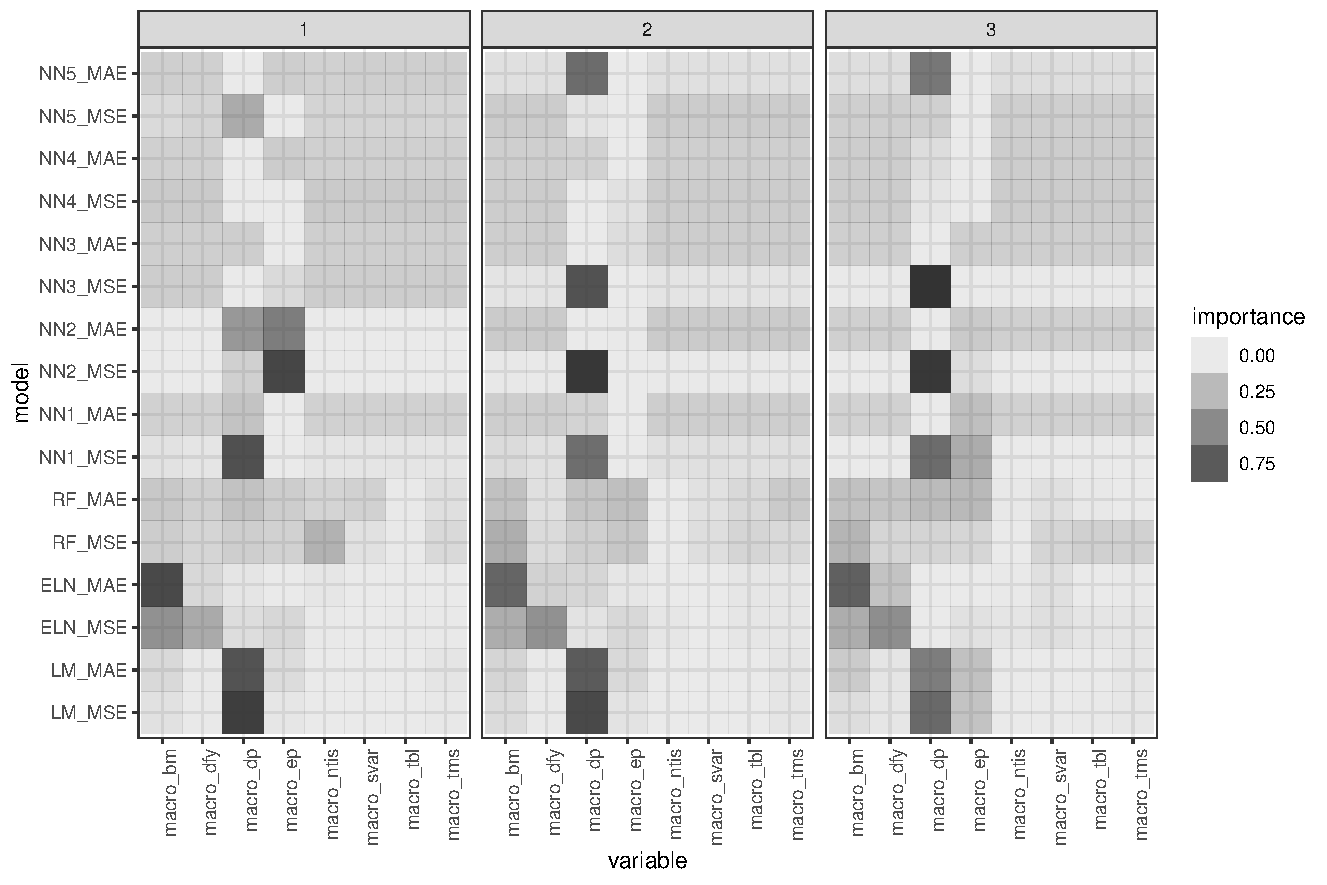
\includegraphics[max size = {\textwidth}{0.35\textheight}]{empirical_sample_all_vi_macro_facet}
	\caption{Empirical Macroeconomic Factor Importance, faceted by training sample}
	\floatfoot{Macroeconomic Factors shown on x axis (see Table \ref{macro_factors} for definitions)}
\end{figure}

If we focus on the two top performing models of elastic net and random forest, we see that they consistently pick out the 1 month and 6 month momentum factors out of the individual characteristics as important, and the book-to-market and default yield spread factors out of the macroeconomic factors are important. In general though, the variable importance metrics are less consistent for the random forests, and it should be noted in particular that the random forest tends to determine factors highly correlated with momentum as important, such as change in moment, dollar trading volume and return volatility. Looking at the macroeconomic factors, penalized linear models tend to identify the average book to market ratio and the default spread as the most important macroeconomic factors. On the macroeconomic factor set, the random forests were inconsistent with the elastic nets, and tended to assign very similar variable importance metrics to most macroeconomic factors.

The neural networks tended to believe that the market value factor was the most important among the individual factors, a result not repeated by any of the other models considered. Within the macroeconomic factors, the neural networks identified and the dividend-price ratio and earnings-price ratio as the most important among the macroeconomic factors, though these results were highly non-robust across different architectures, loss functions and training samples.

Interestingly, we find that the linear models assign the controversial dividend price ratio macroeconomic factor as highly important, a result mirrored only with the neural networks Their variable importance for individual factors across different training samples is highly non-robust, with the important variables almost completely changing year to year. The linear models consistently identified the controversial dividend-price ratio as important, a result that was somewhat consistent with the neural networks. 

The overall results again contradict the results of \cite{gu_empirical_2018}, who conclude that all of the machine methods agree on the same subset of important factors. Indeed, we only see consistency in variable importance between the elastic nets and random forests on the individual factors only - all other variable importance metrics were either inconsistent between different models, or non-robust.

All models considered typically preferred sparse parameterizations. That is, most if not all of the individual factors had little to no importance across all models.\footnote{Note that because the variable importance here was not evaluated explicitly for each pairwise interaction term, some of the individual factors appear as slightly important. This is because setting an individual factor to zero also sets some of the macroeconomic pairwise terms to zero, increasing its apparent importance.}




\end{document}